\chapter{Turbulent profiles}
\label{app:turbulentProfiles}

This section contains some complementary graphs for turbulent simulations that have not been shown in the main text, but can be interesting to extend the discussion. 

\section{Mid-plane plots for density}
\label{sec:turbulentProfiles_CIRC}

\begin{figure}[H]\centering
	\begin{subfigure}[t]{0.45\textwidth}
		\centering
		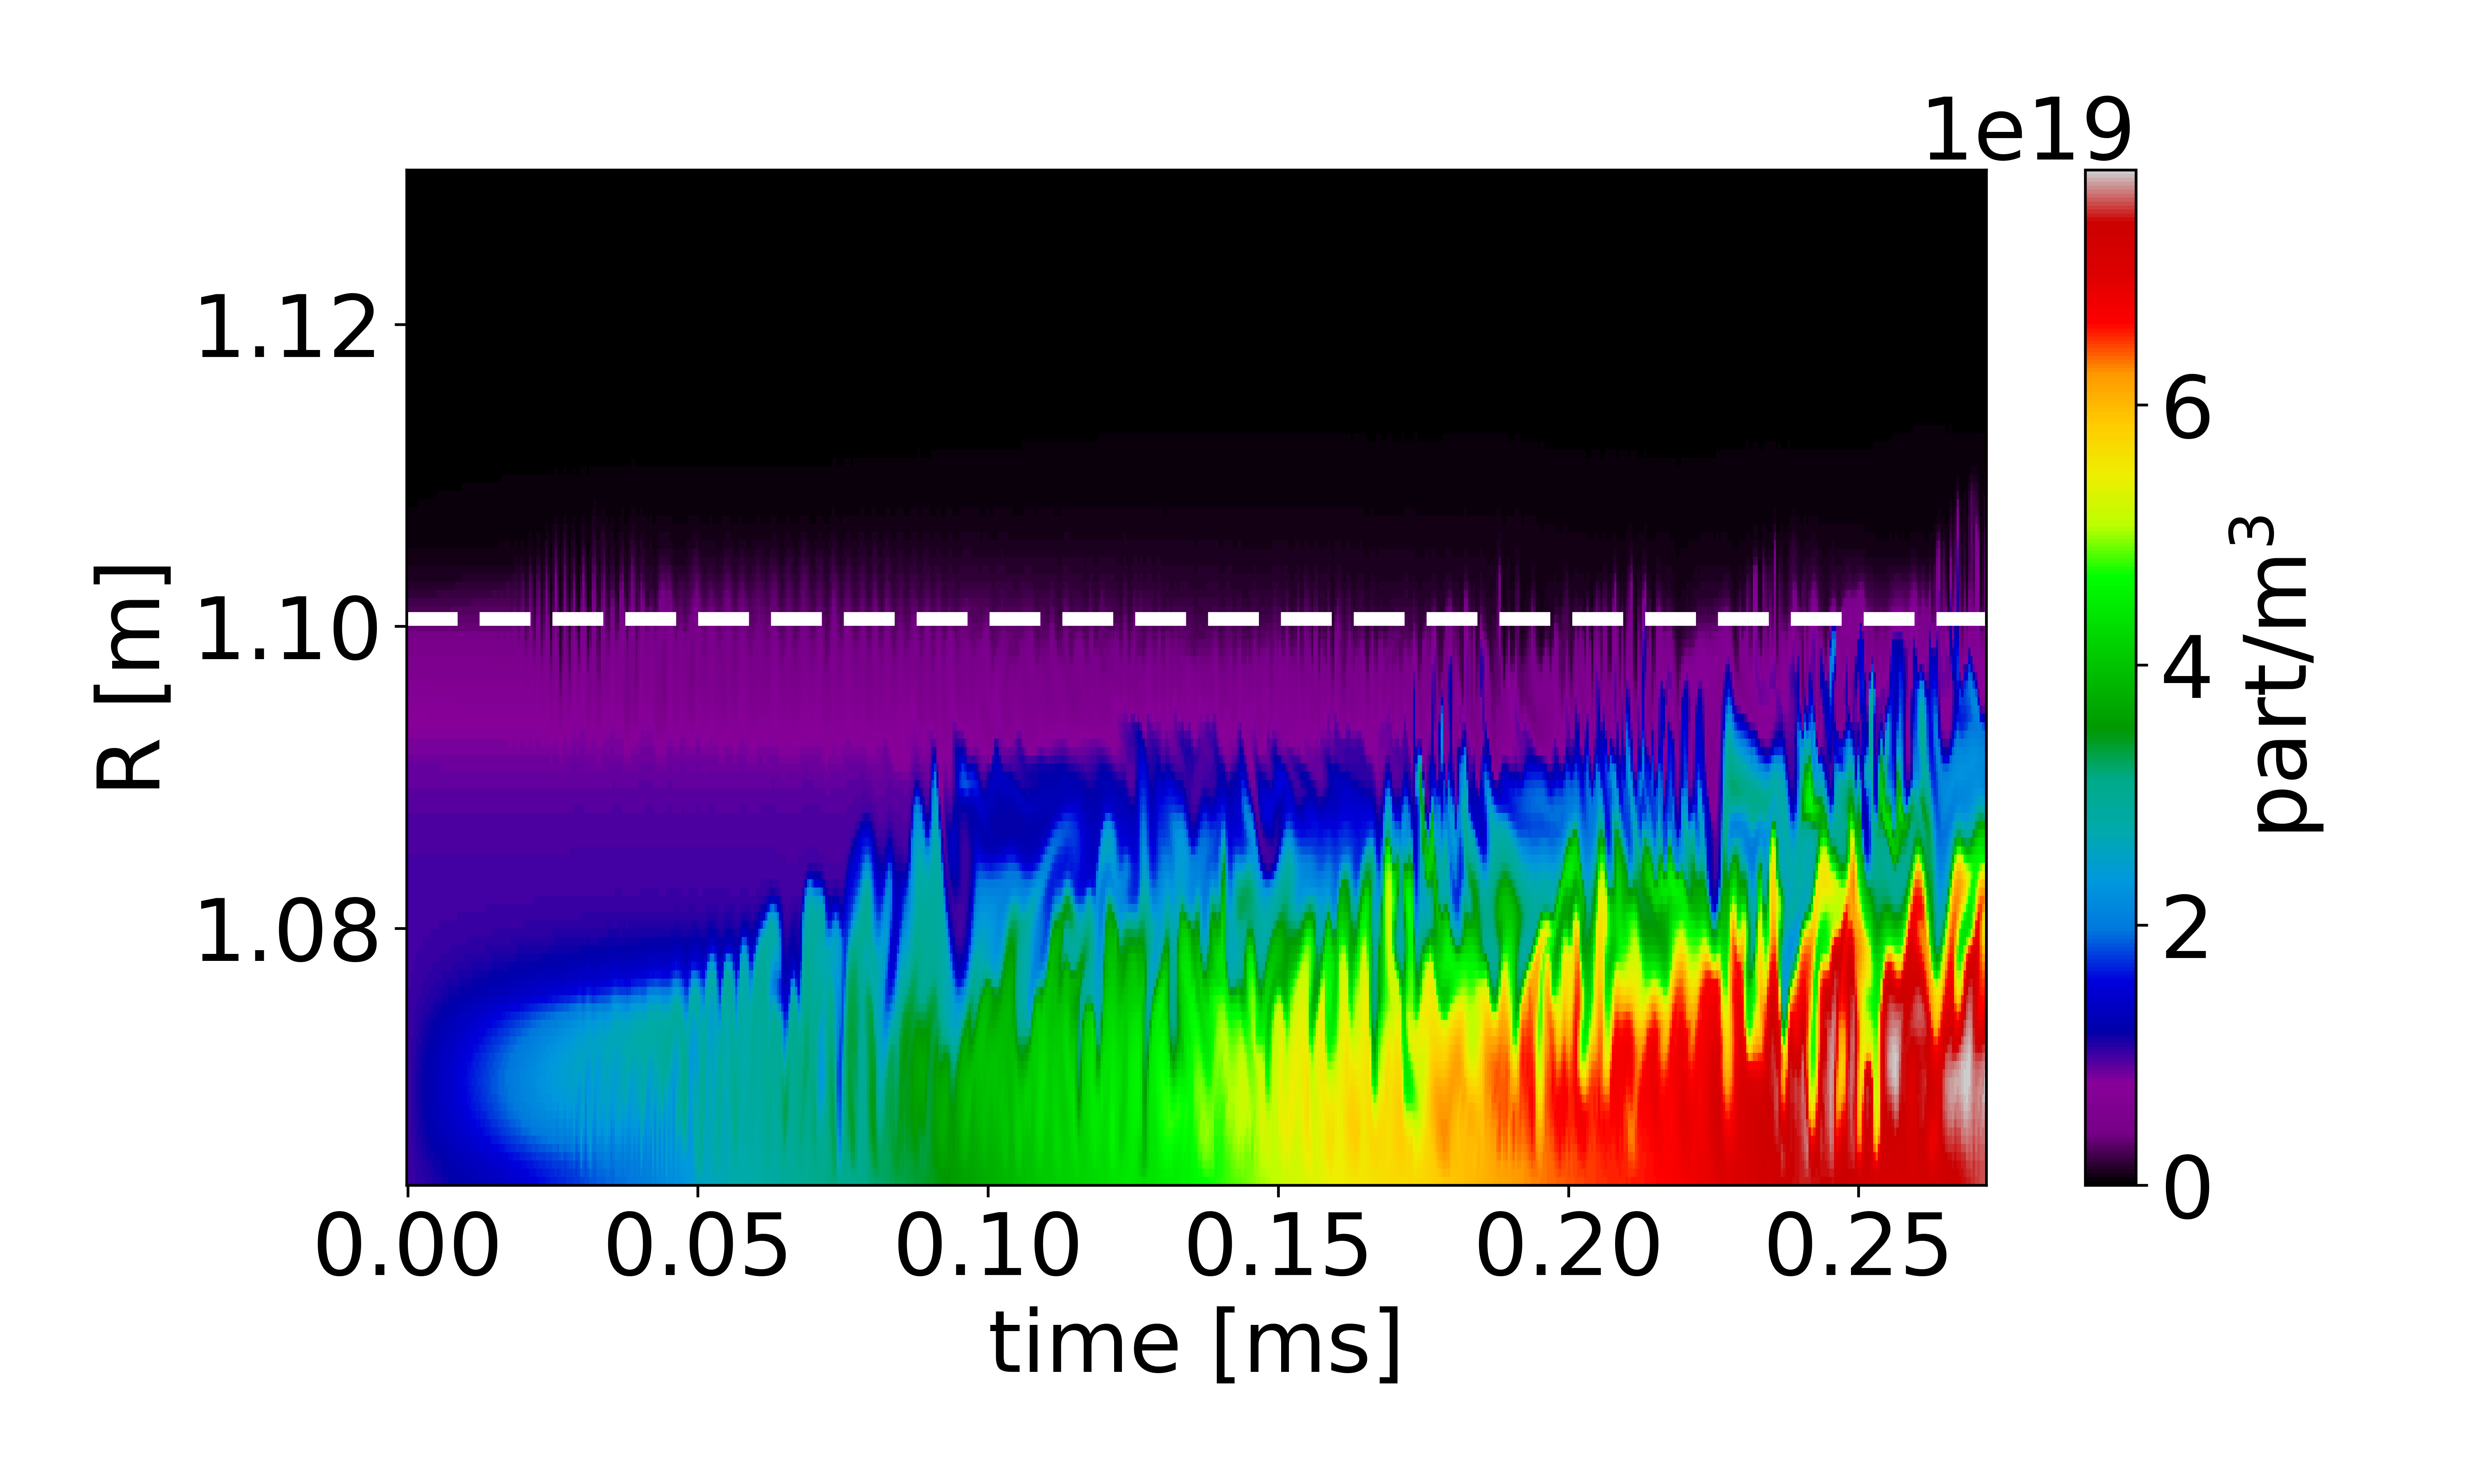
\includegraphics[width=1\textwidth]{schemes/plotOMPtime_spec1_n_PHI.jpg}
		\subcaption{Electrostatic - ion density}
	\end{subfigure}
	\begin{subfigure}[t]{0.45\textwidth}
		\centering
		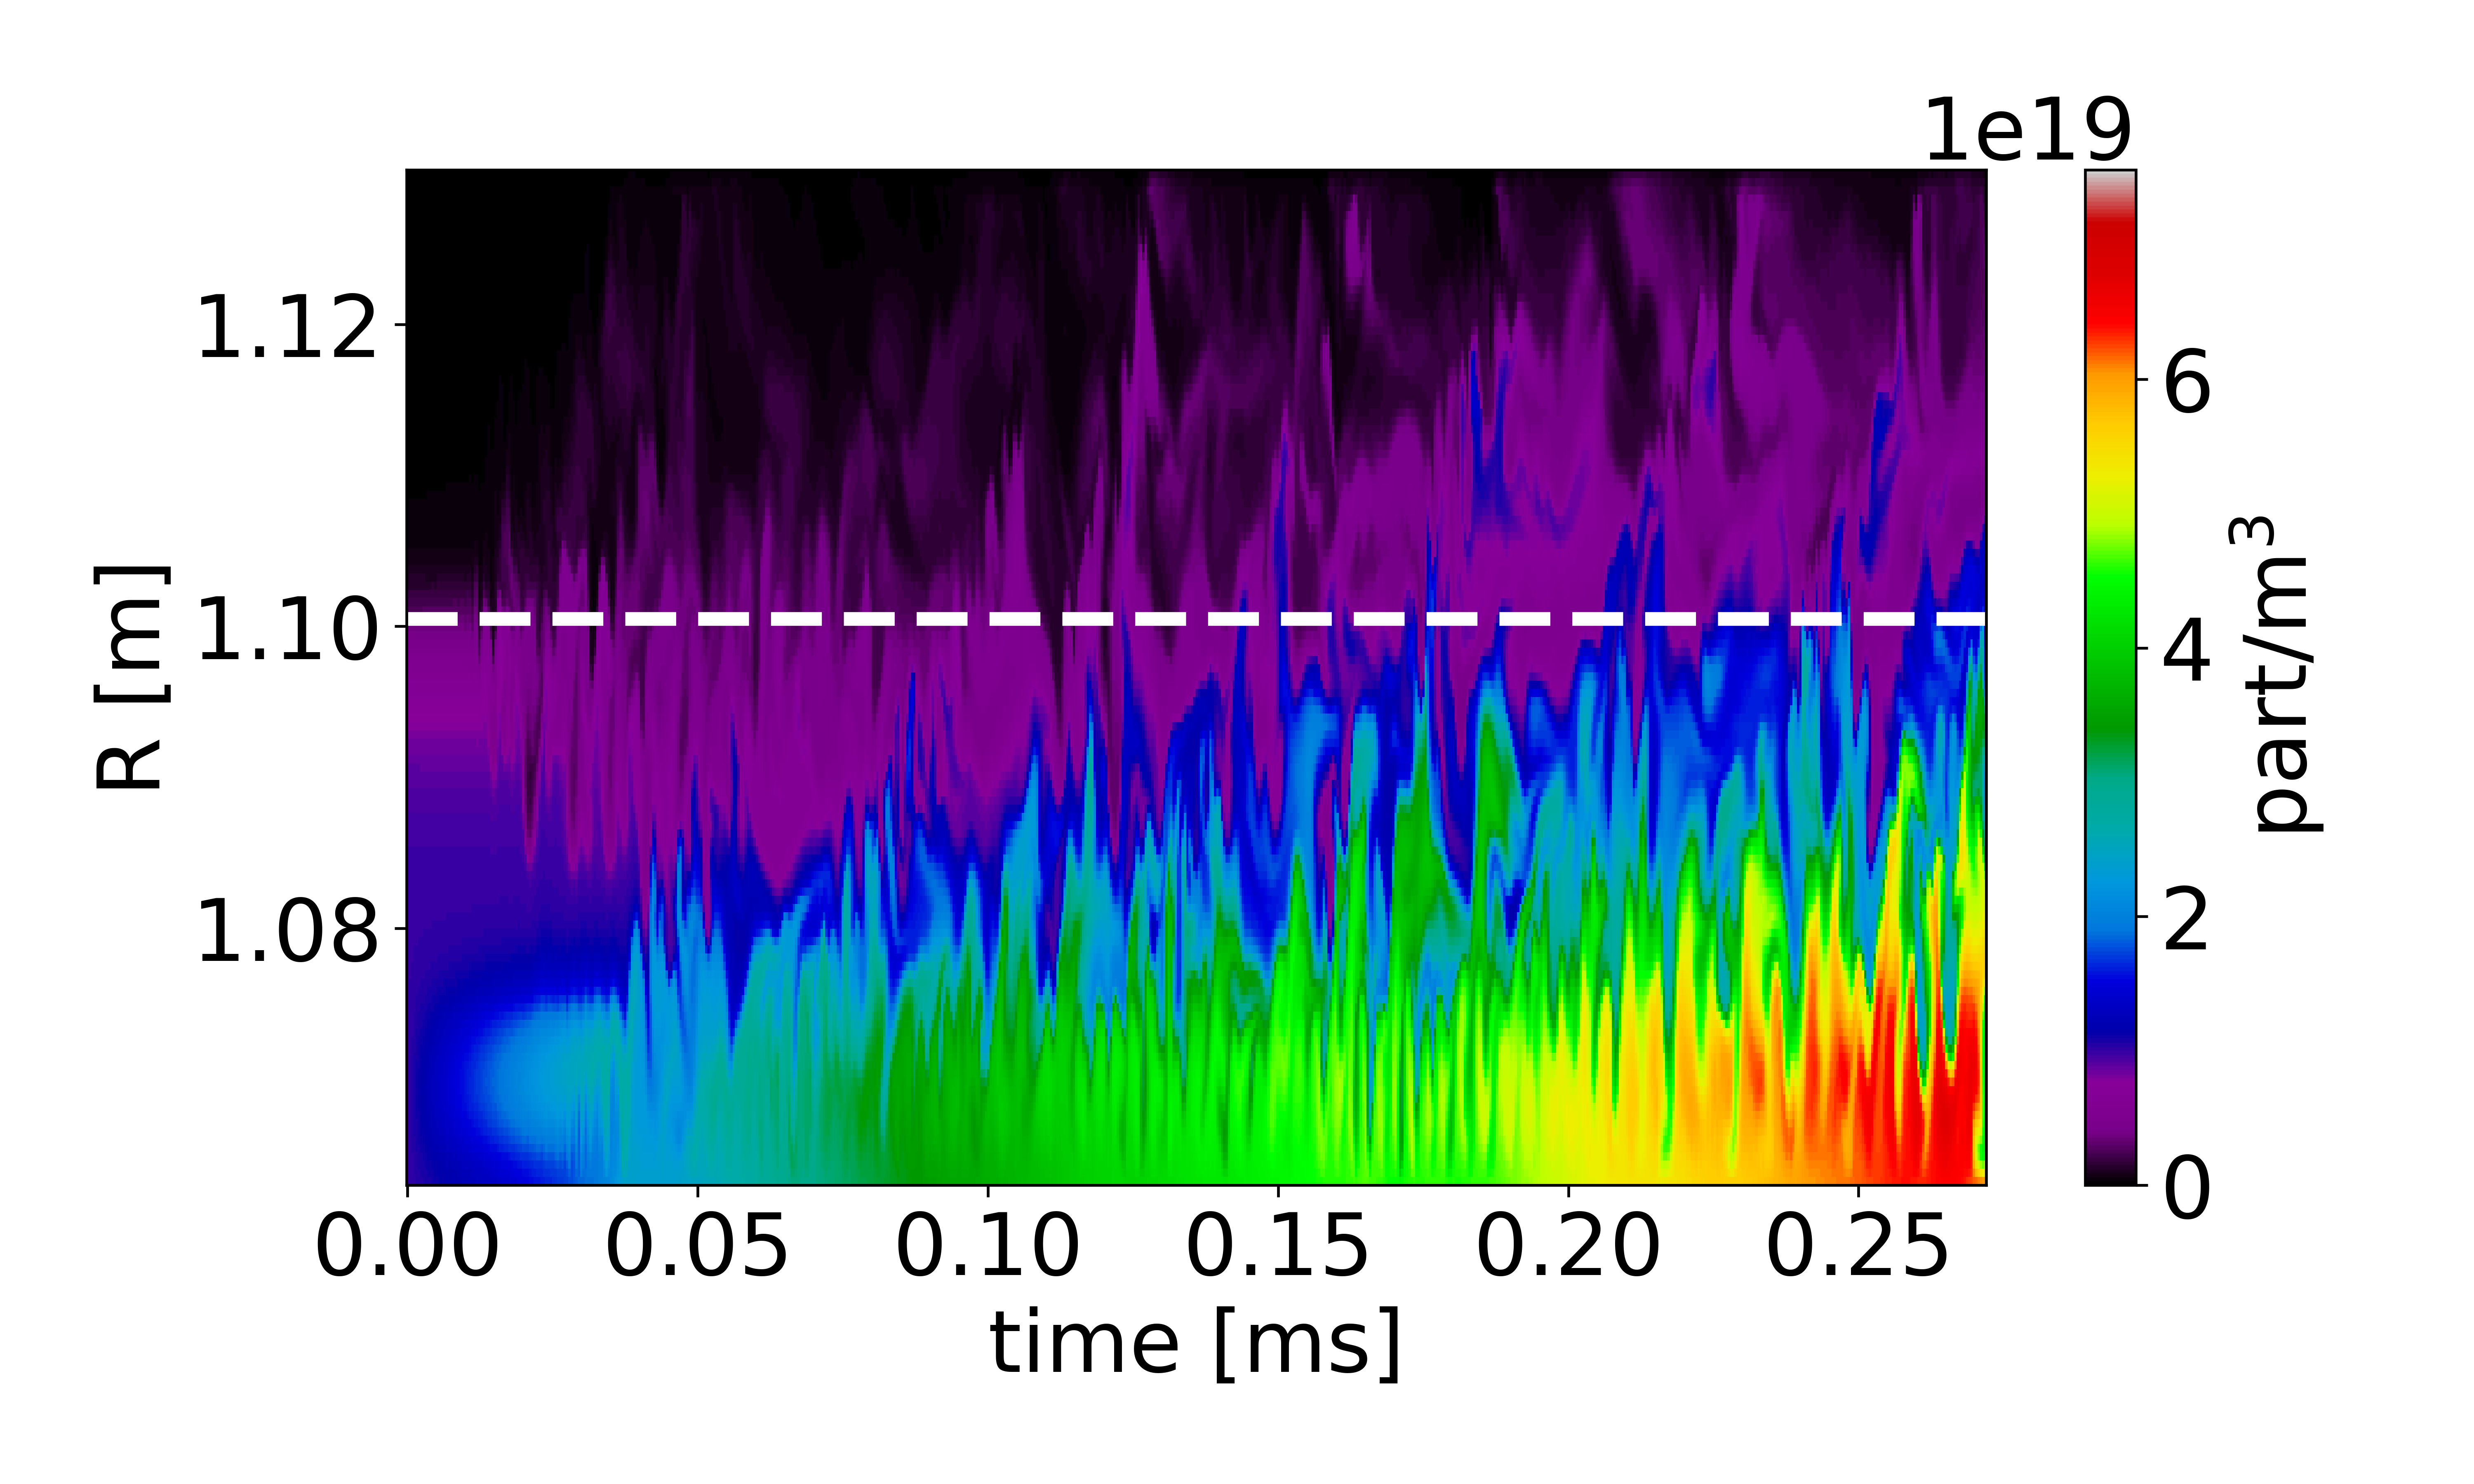
\includegraphics[width=1\textwidth]{schemes/plotOMPtime_spec1_n_PHIJ_mass_1.jpg}
		\subcaption{Electron inertia - ion density}
	\end{subfigure}
	\begin{subfigure}[t]{0.45\textwidth}
		\centering
		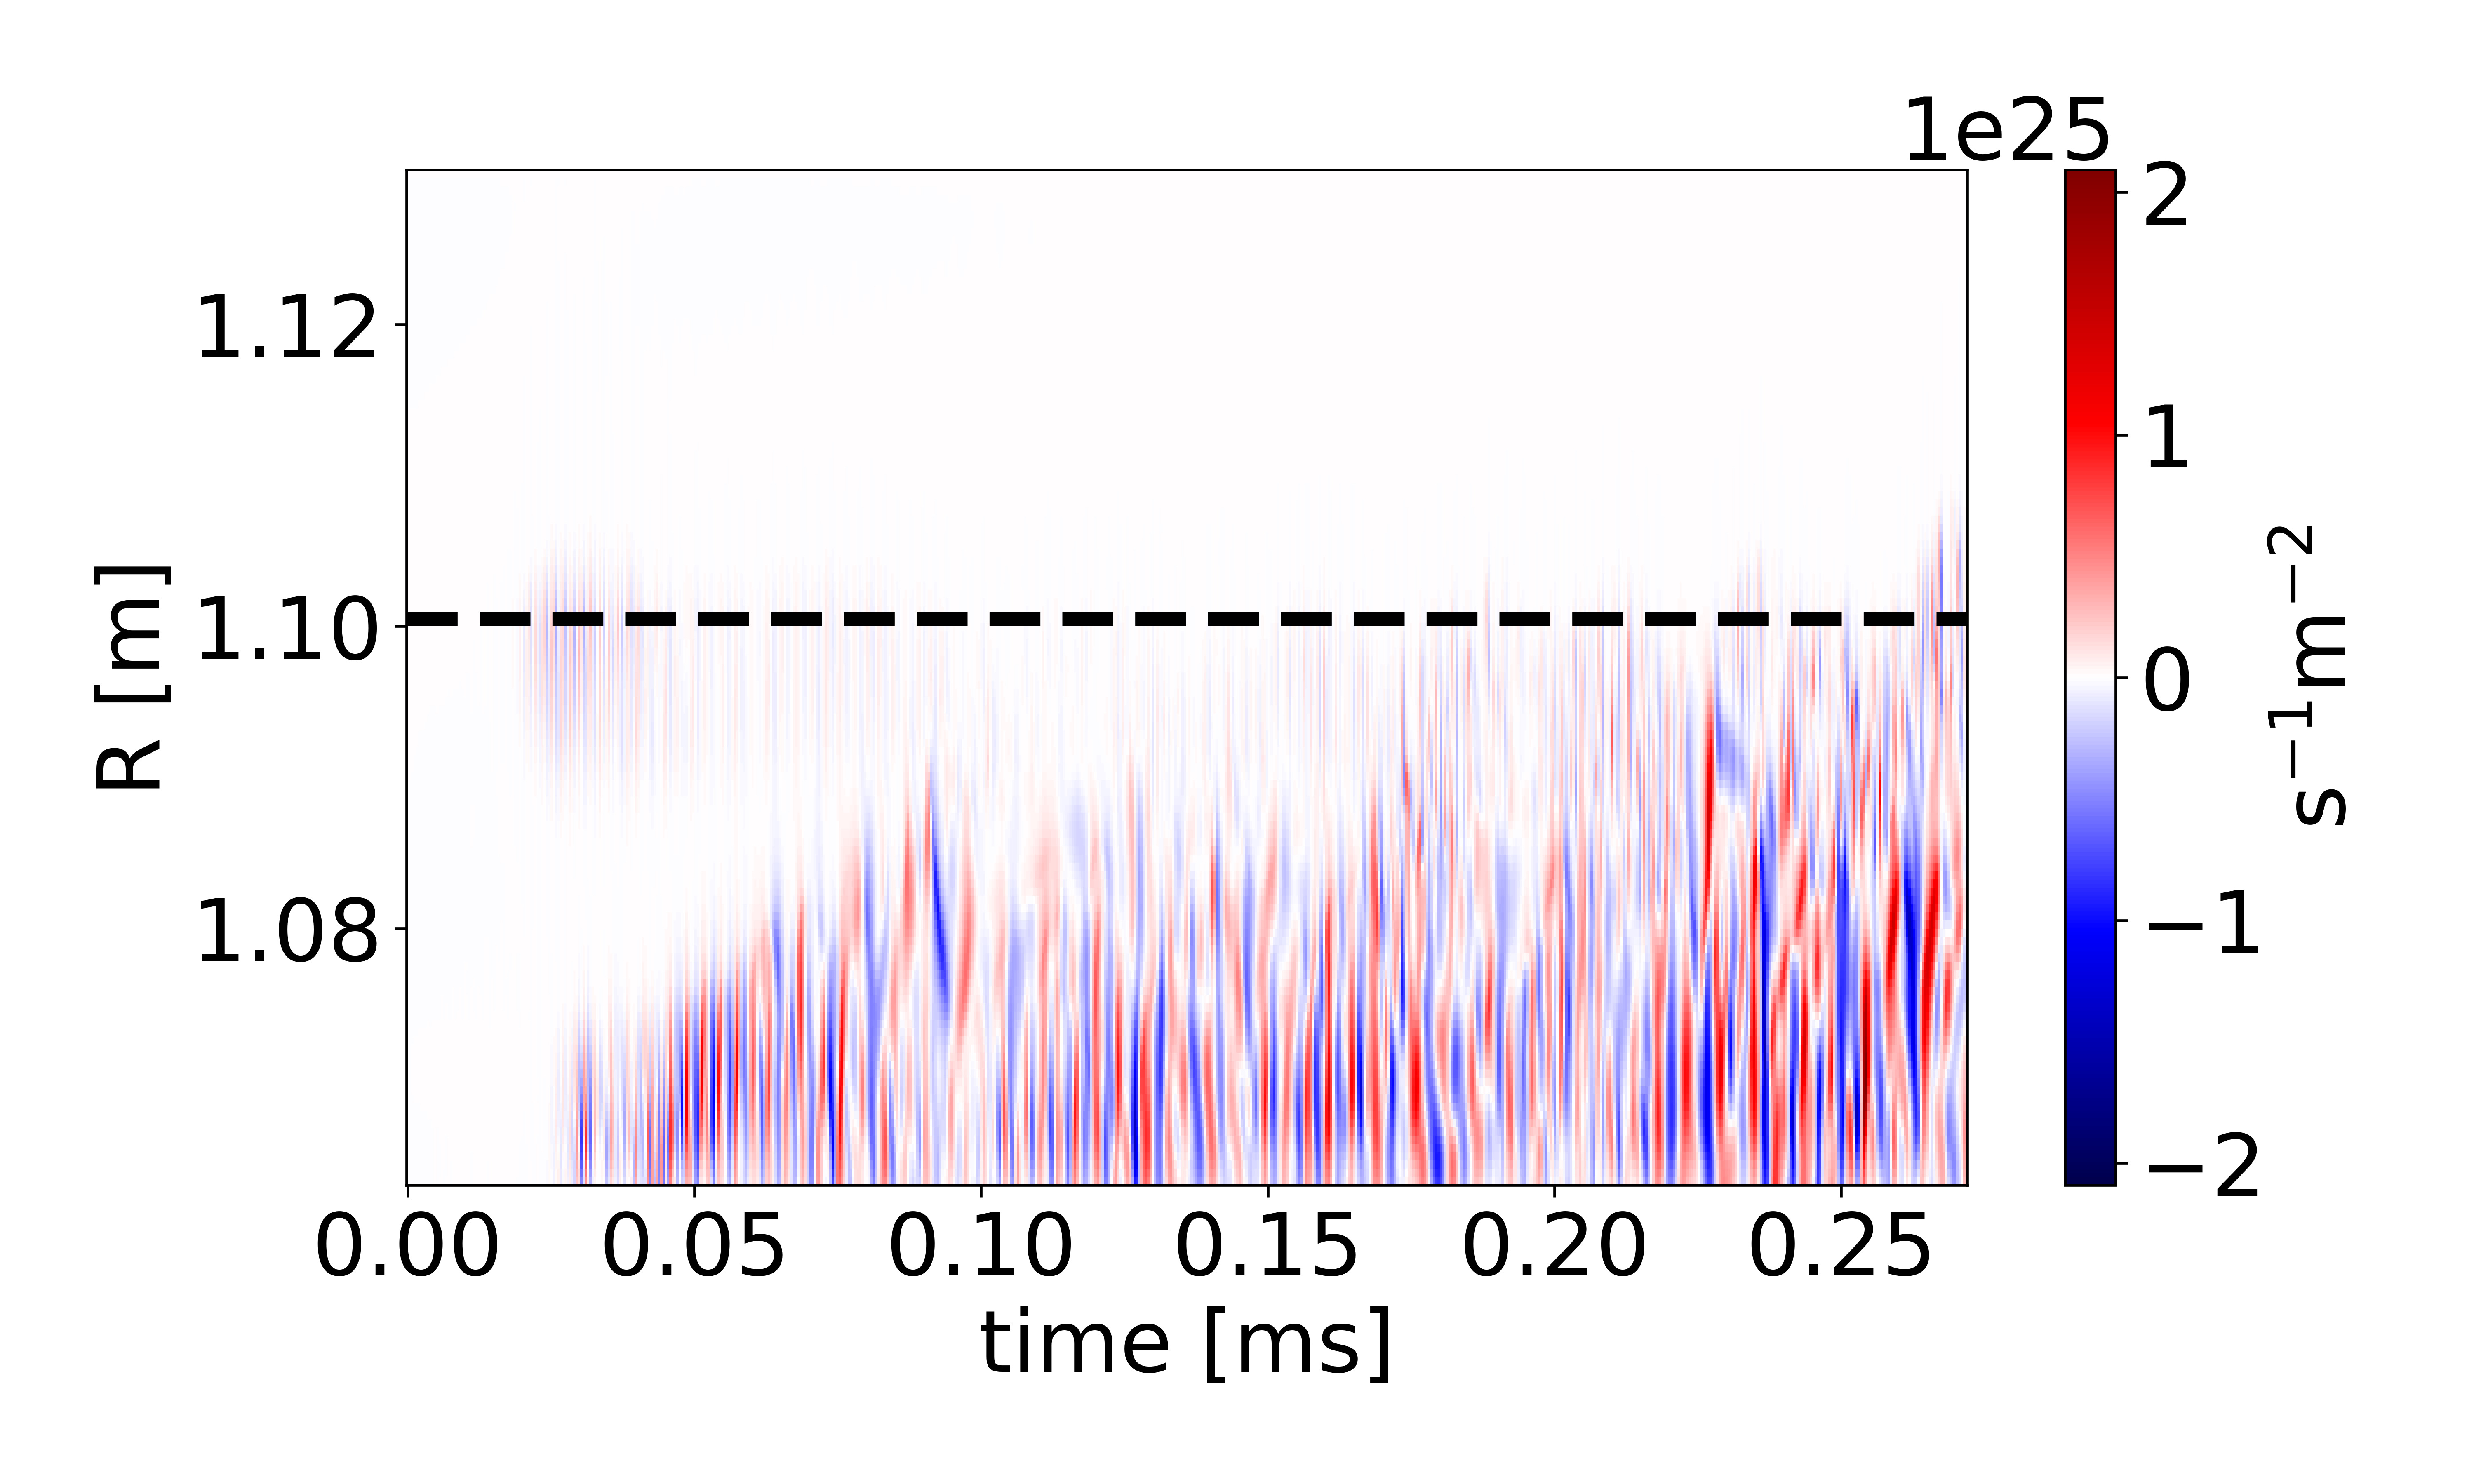
\includegraphics[width=1\textwidth]{schemes/plotOMPtime_spec1_fluxn_psi_PHI.jpg}
		\subcaption{Electrostatic - radial particle flux}
	\end{subfigure}
	\begin{subfigure}[t]{0.45\textwidth}
		\centering
		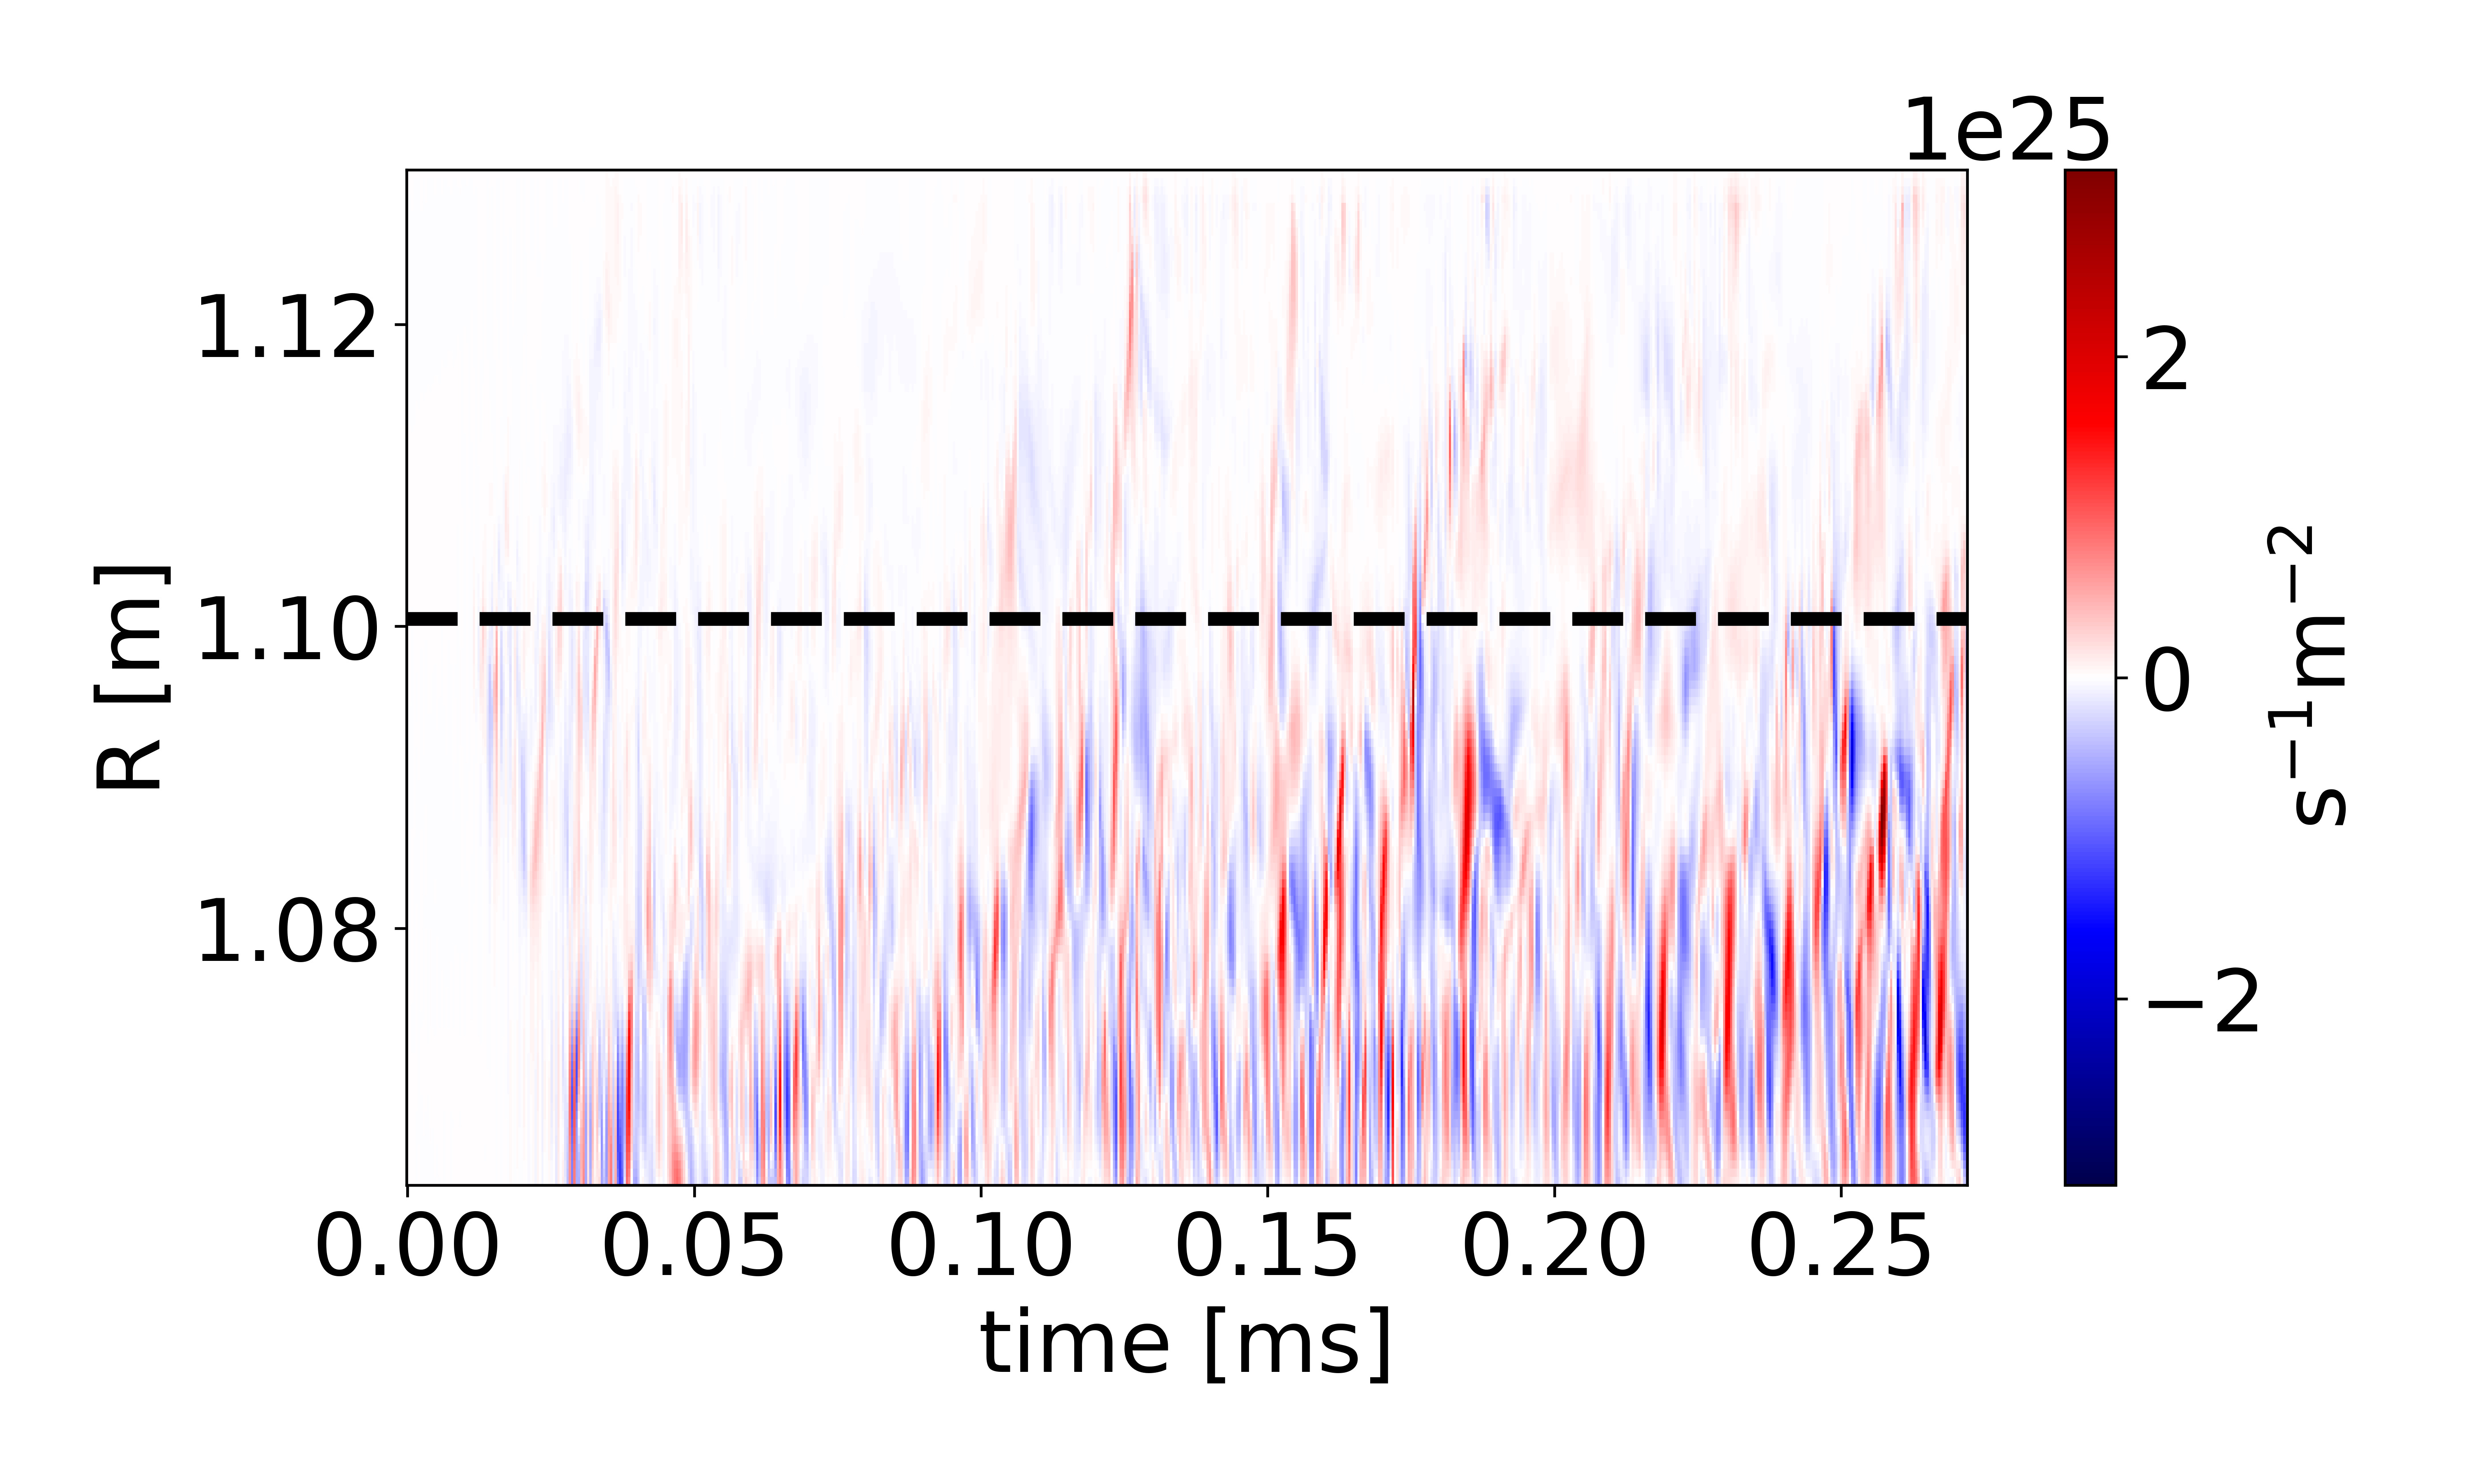
\includegraphics[width=1\textwidth]{schemes/plotOMPtime_spec1_fluxn_psi_PHIJ_mass_1.jpg}
		\subcaption{Electron inertia - radial particle flux}
	\end{subfigure}
	\caption{Evolution of the radial ion density profiles and particle fluxes at the outer mid-plane for the electrostatic scenarios. The dashed line indicates the position of the separatrix and the plasma in the first poloidal plane is taken}
	\label{fig:CIRC_EI_OMPevolution_n}
\end{figure}

\begin{figure}[H]\centering
	\begin{subfigure}[t]{0.45\textwidth}
		\centering
		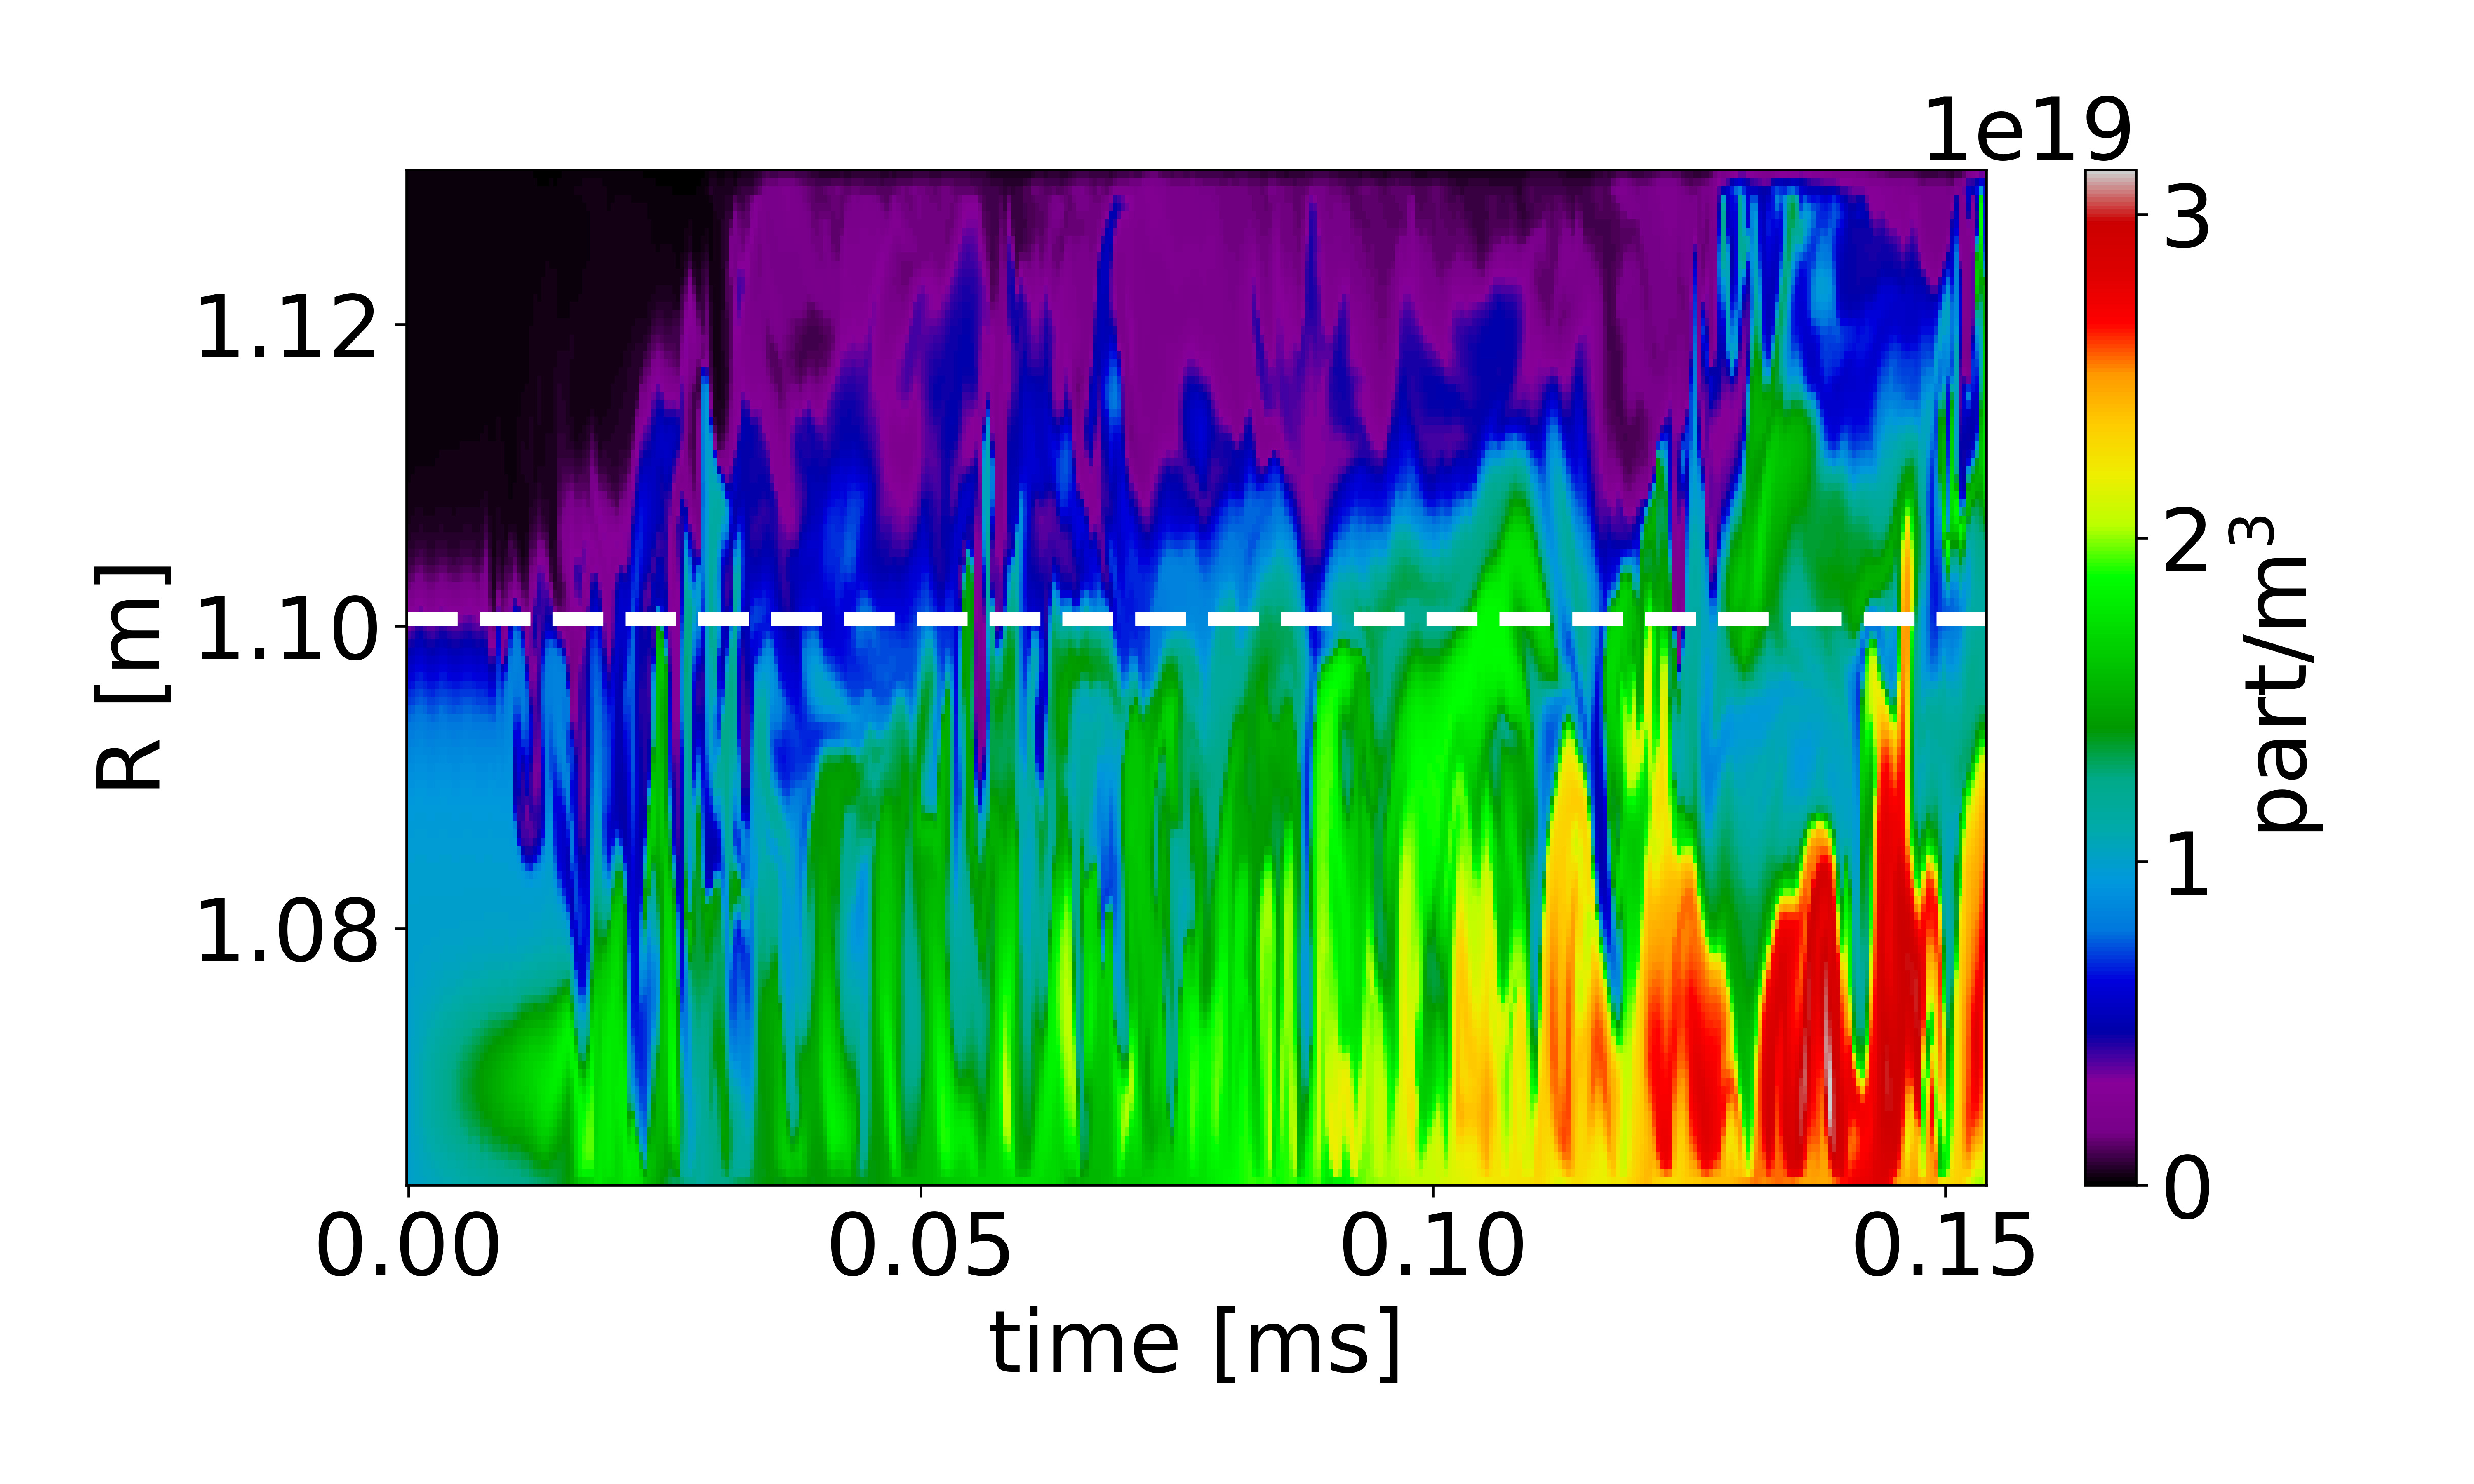
\includegraphics[width=1\textwidth]{schemes/plotOMPtime_spec1_n_PHIAJ_beta_1.jpg}
		\subcaption{Electromagnetic - ion density}
	\end{subfigure}
	\begin{subfigure}[t]{0.45\textwidth}
		\centering
		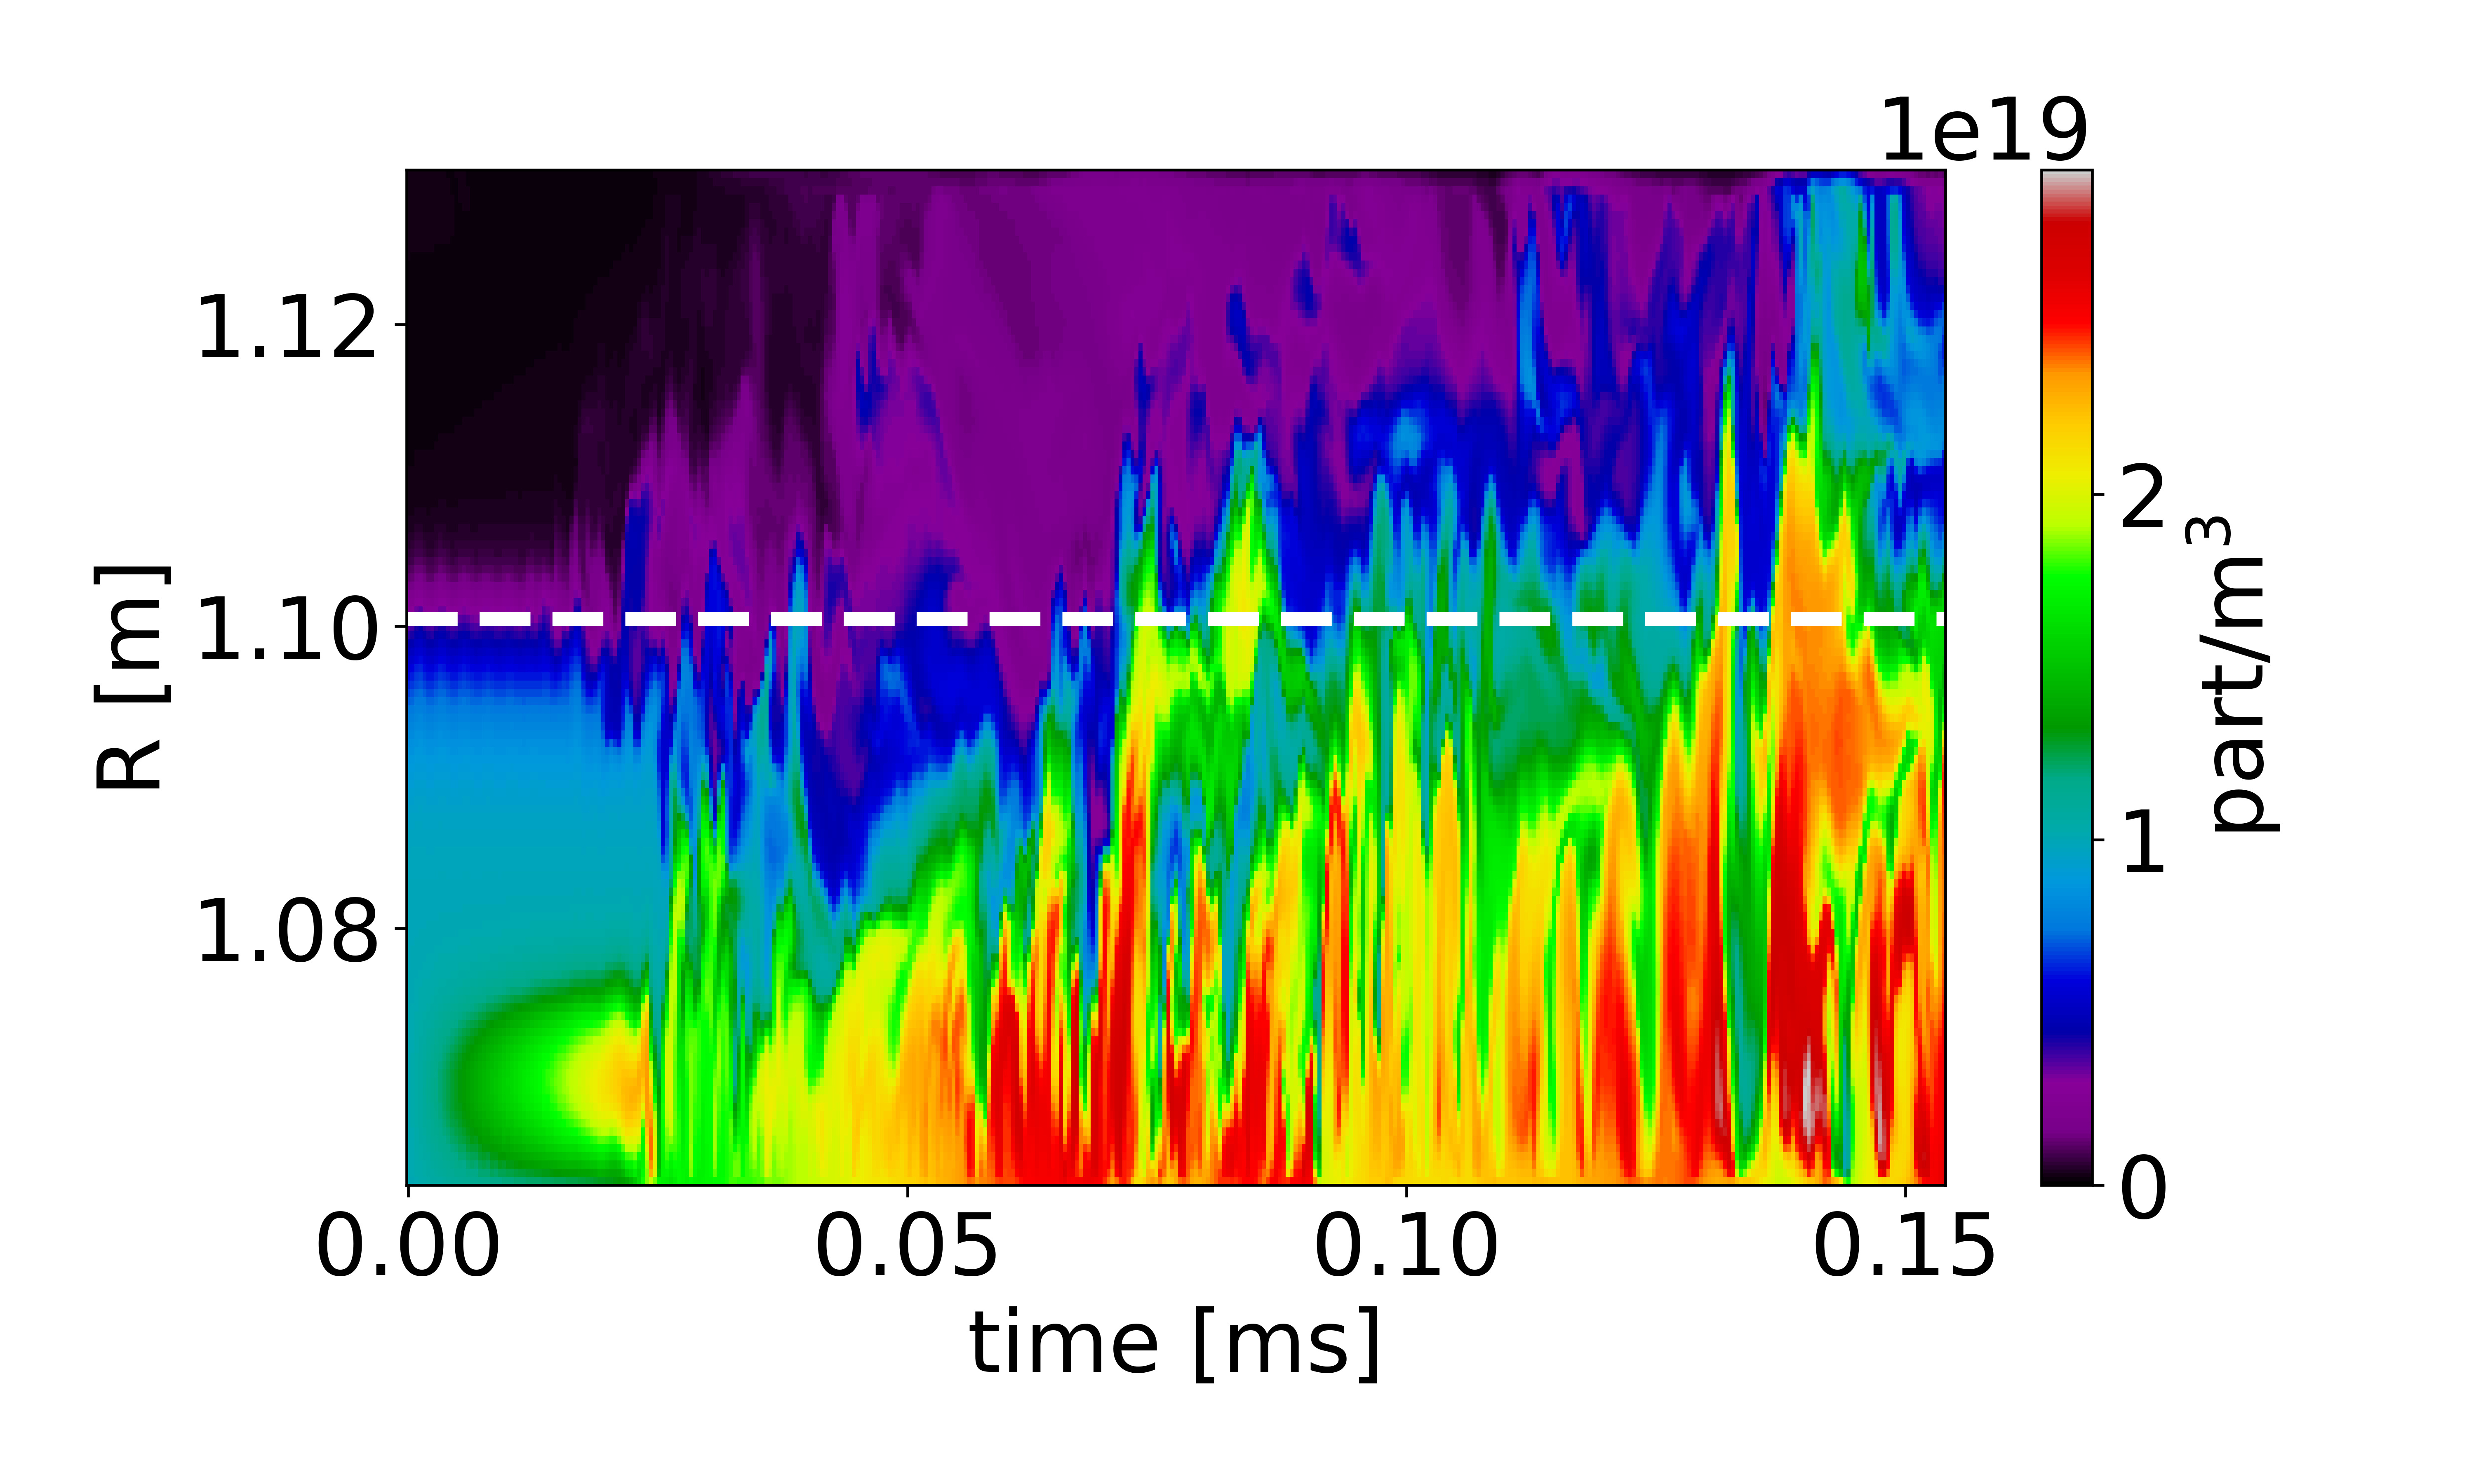
\includegraphics[width=1\textwidth]{schemes/plotOMPtime_spec1_n_flutter.jpg}
		\subcaption{Electromagnetic with flutter - ion density}
	\end{subfigure}
	\begin{subfigure}[t]{0.45\textwidth}
		\centering
		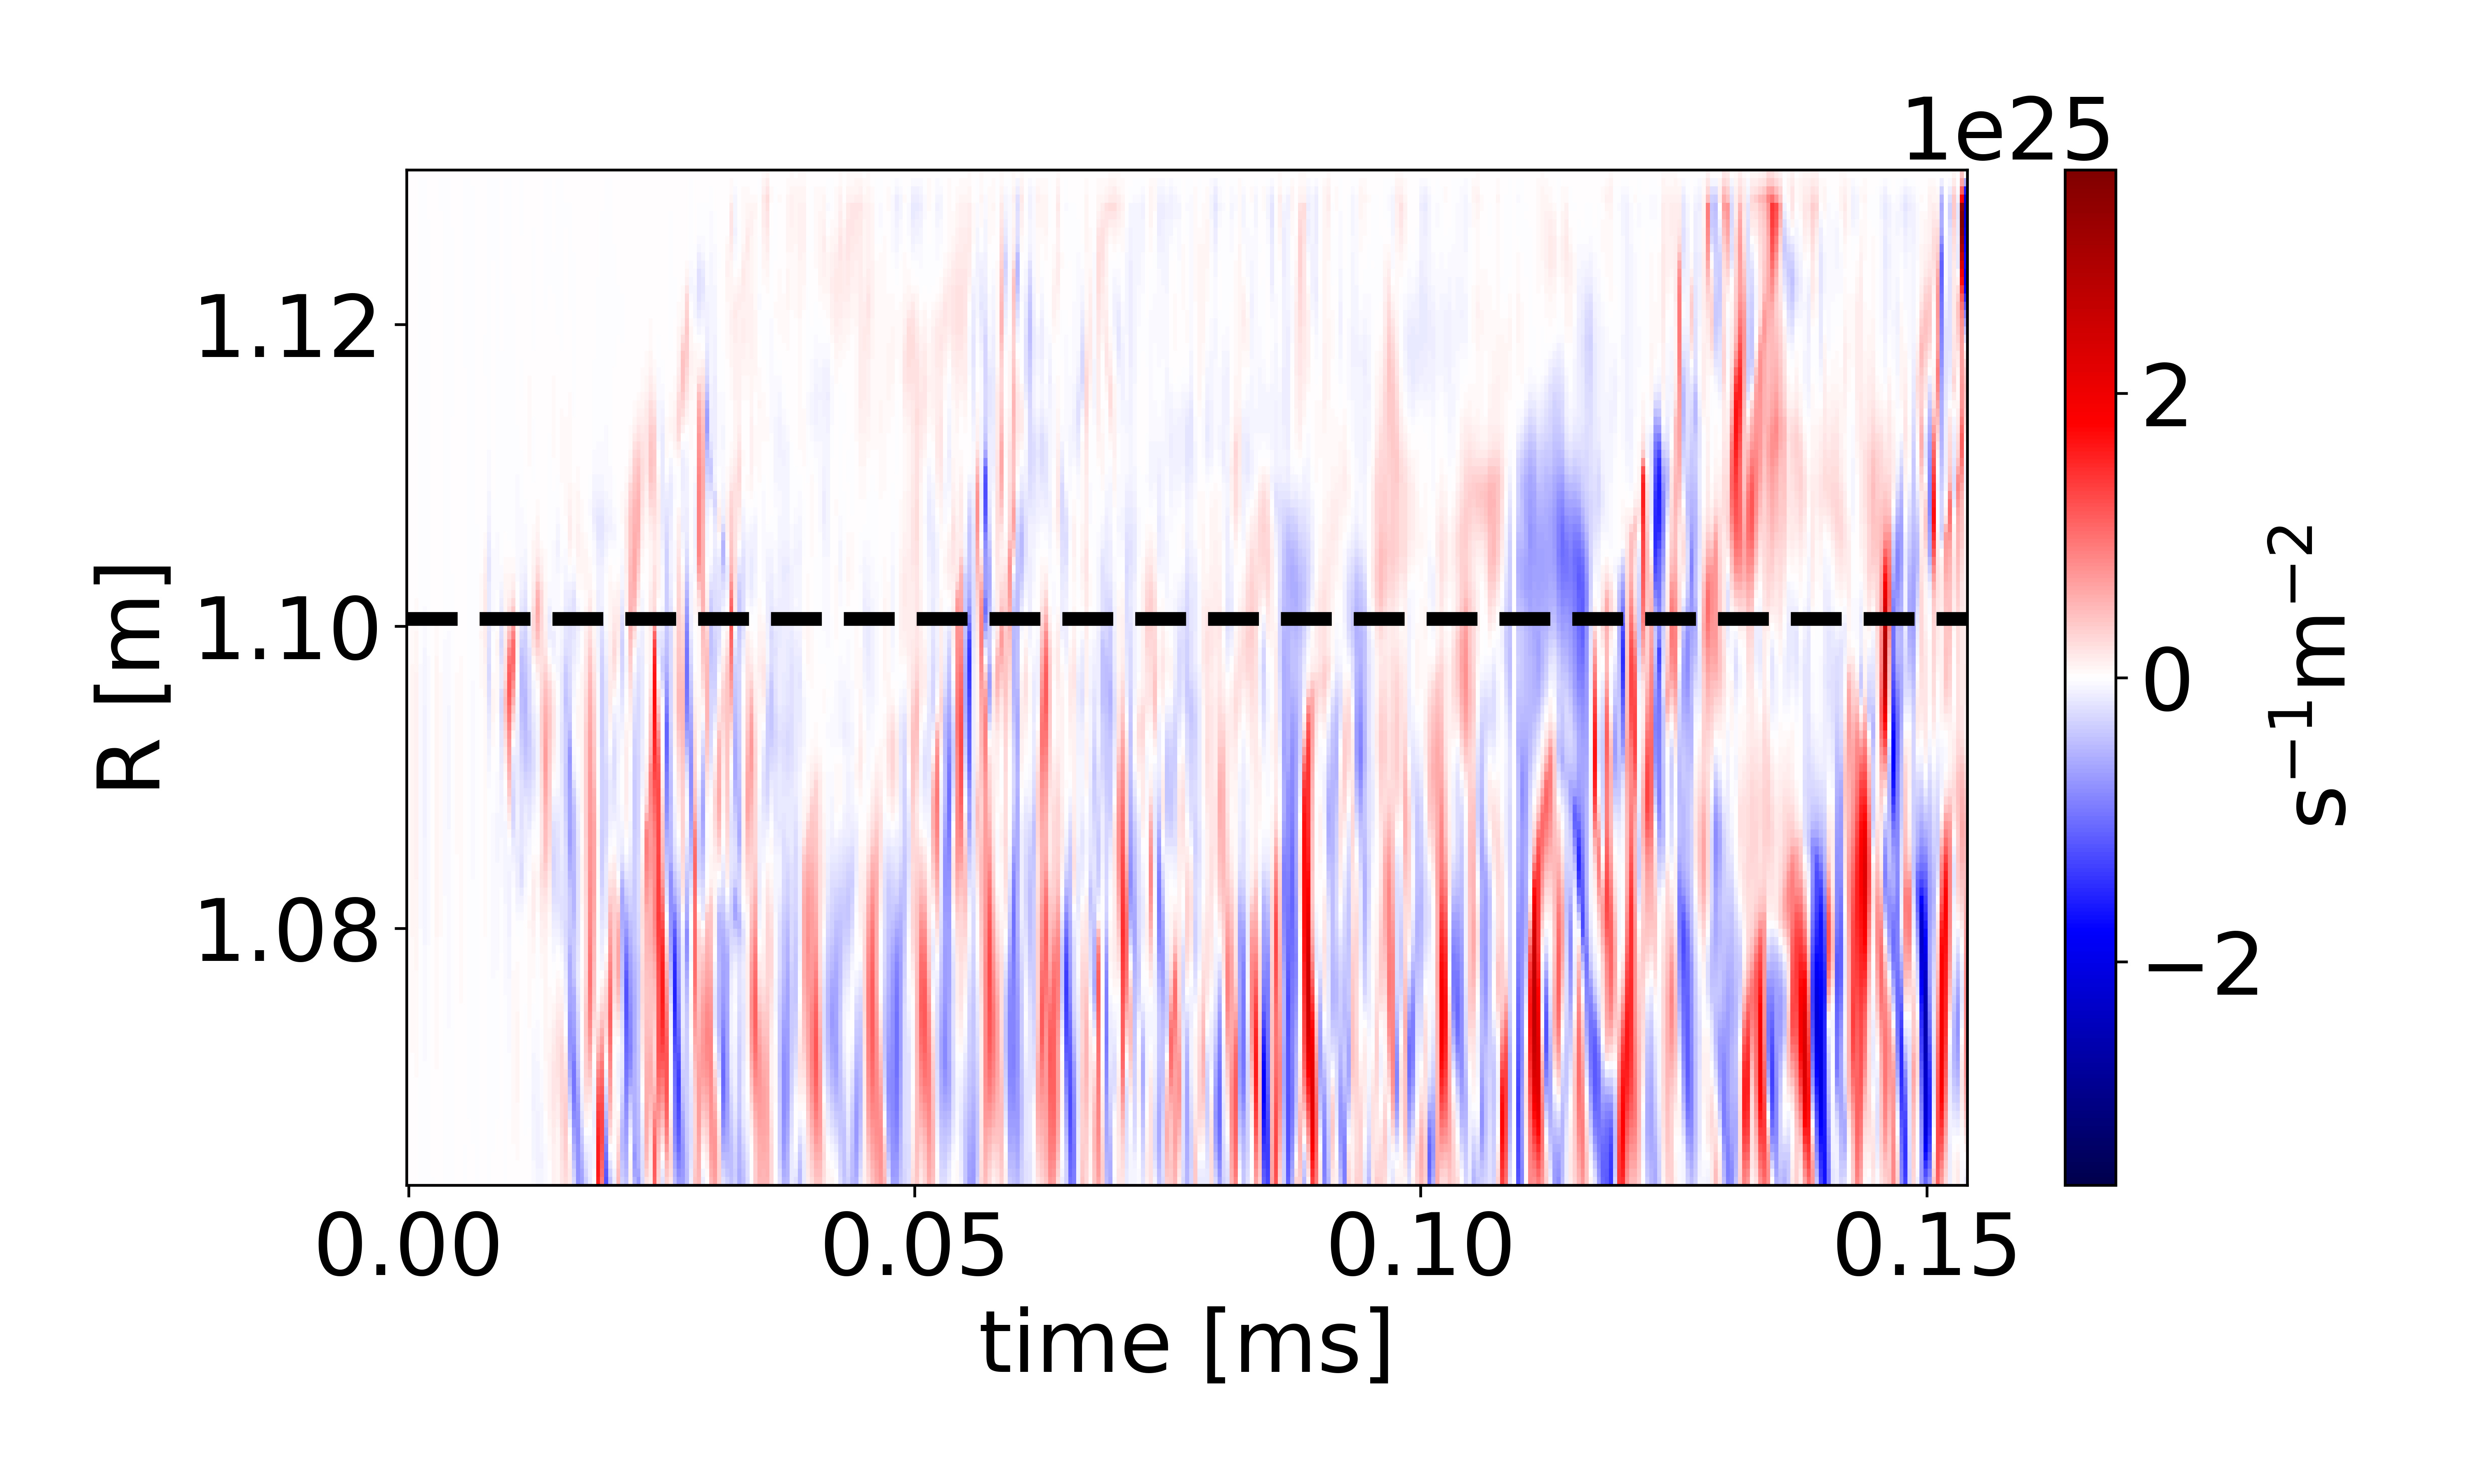
\includegraphics[width=1\textwidth]{schemes/plotOMPtime_spec1_fluxn_psi_PHIAJ_beta_1.jpg}
		\subcaption{Electromagnetic - radial particle flux}
	\end{subfigure}
	\begin{subfigure}[t]{0.45\textwidth}
		\centering
		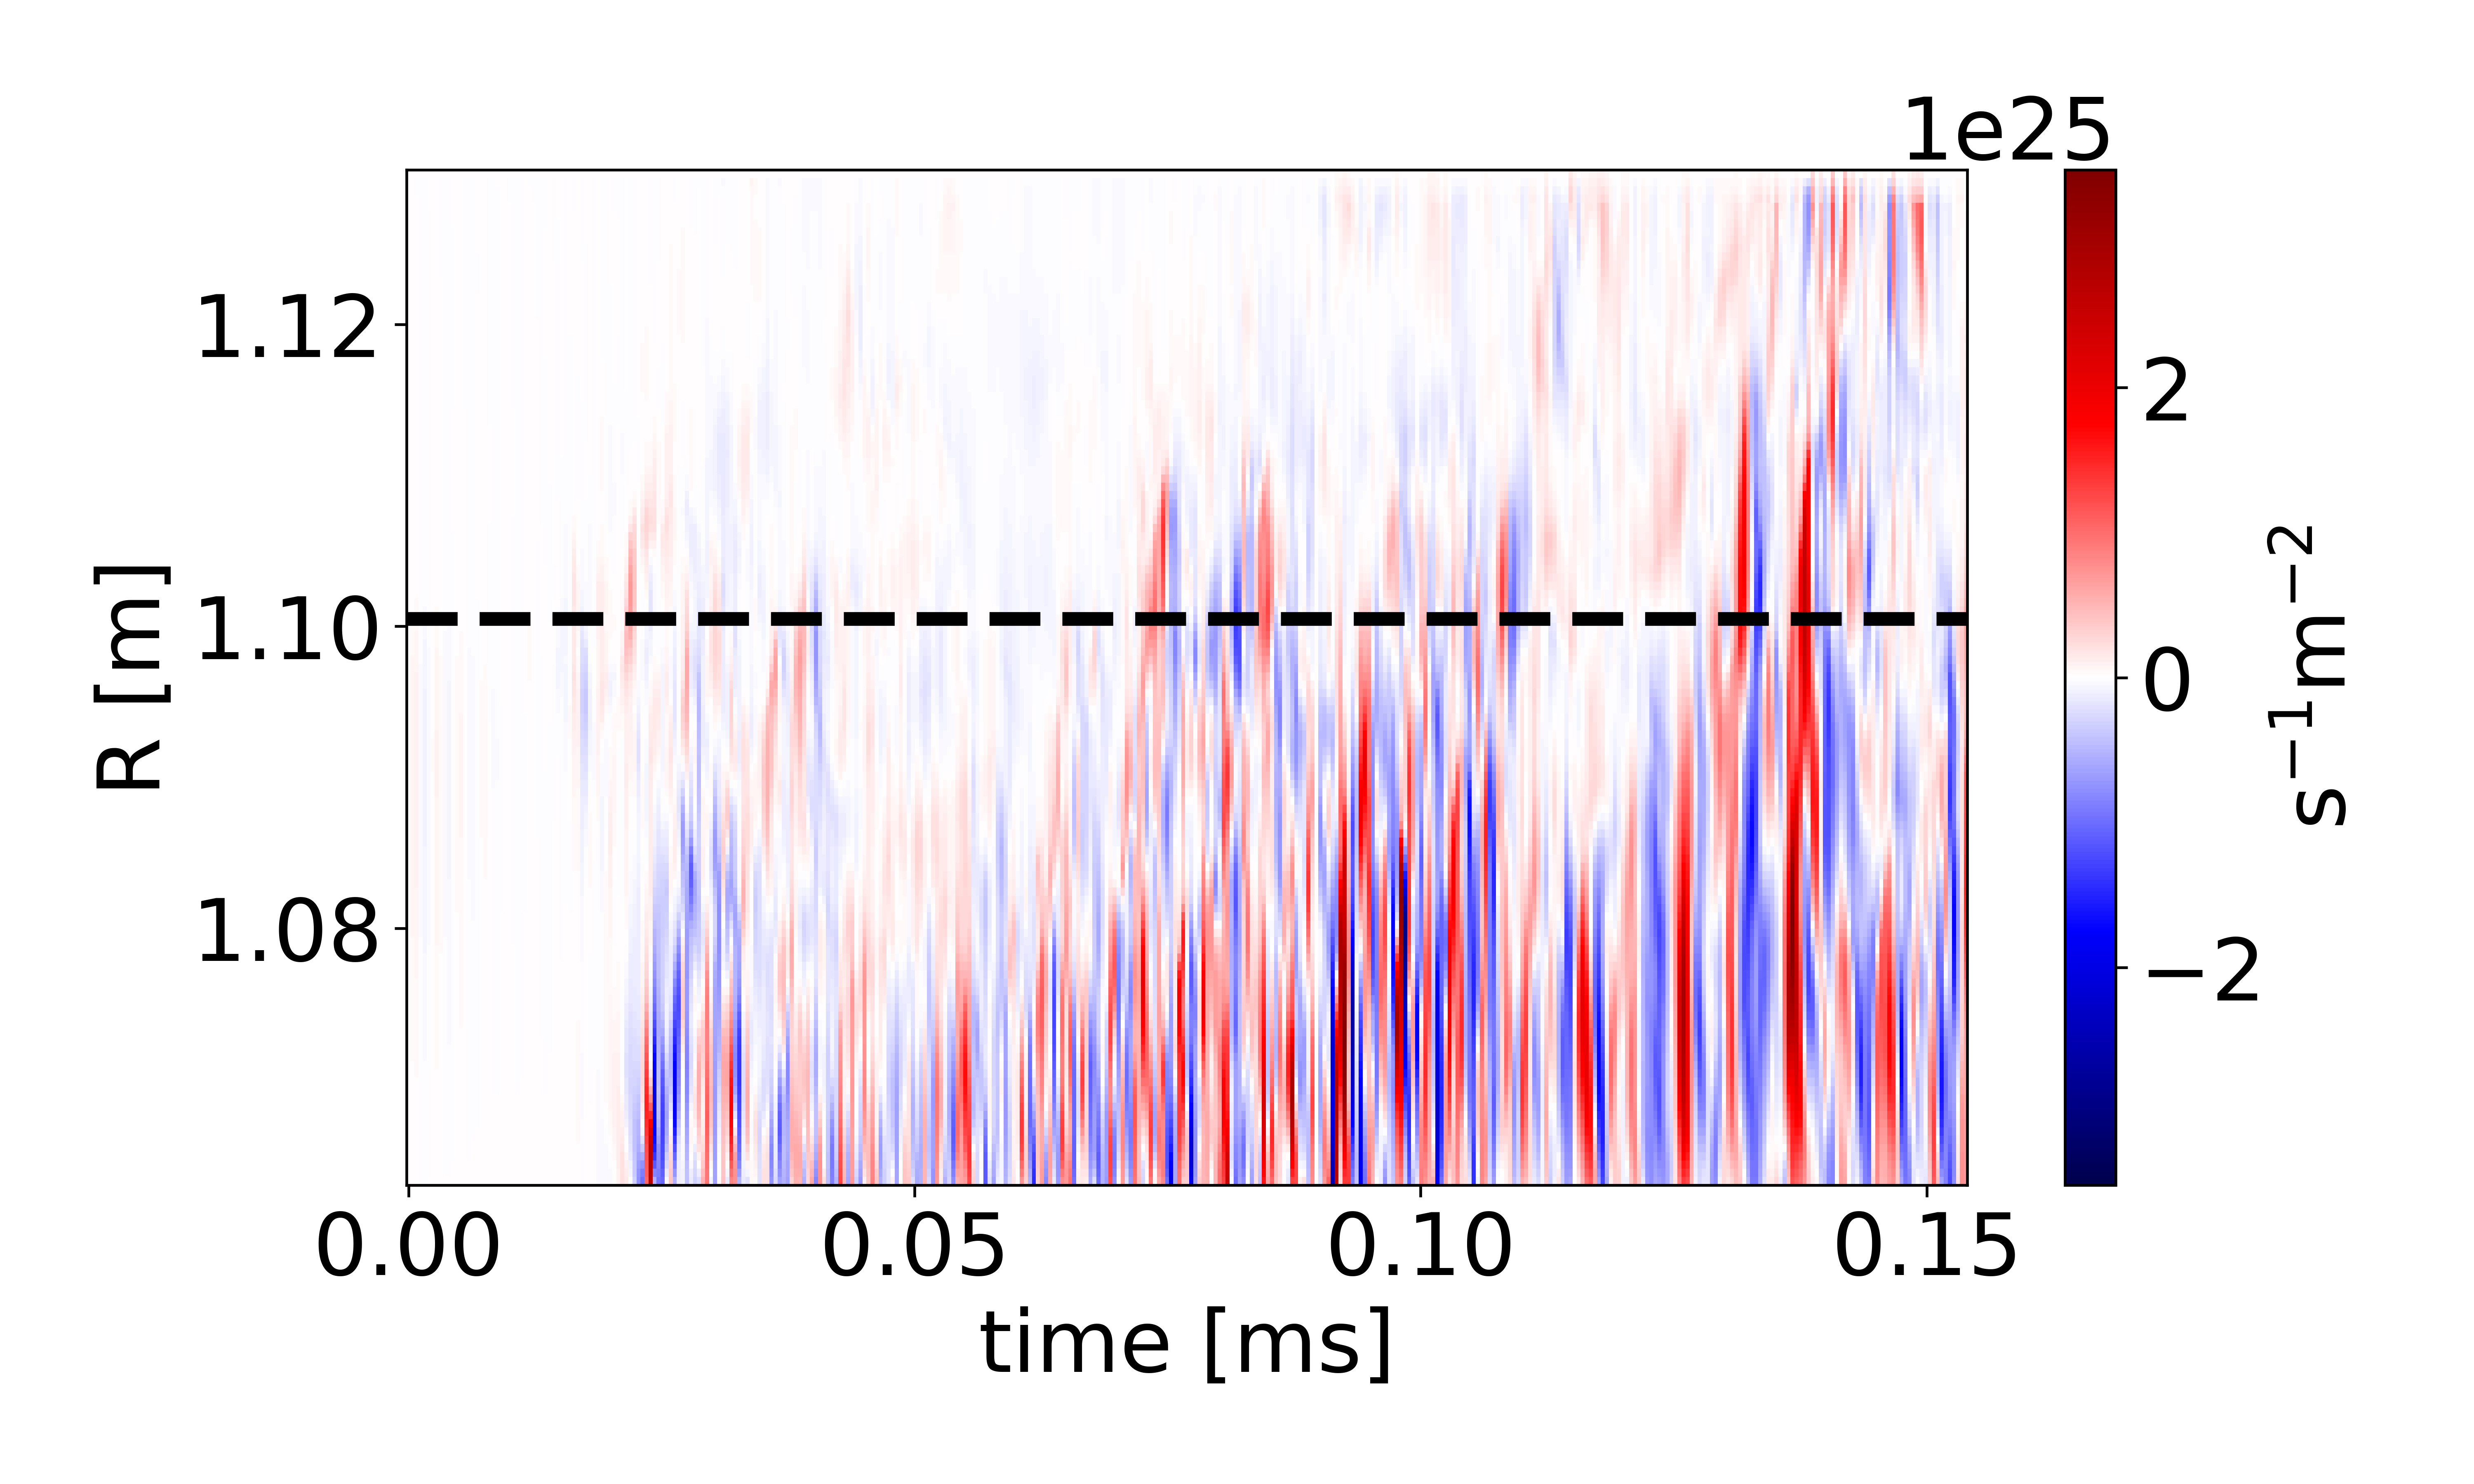
\includegraphics[width=1\textwidth]{schemes/plotOMPtime_spec1_fluxn_psi_flutter.jpg}
		\subcaption{Electromagnetic with flutter - radial particle flux}
	\end{subfigure}
	\caption{Evolution of the radial ion density profiles and particle fluxes at the outer mid-plane for the electromagnetic scenarios. The dashed line indicates the position of the separatrix and the plasma in the first poloidal plane is taken}
	\label{fig:CIRC_EM_OMPevolution_n}
\end{figure}


\section{Perpendicular modes on for electron inertia and magnetic induction on the circular scenario}
\label{sec:turbulentProfiles_CIRCmodal}


\begin{figure}[H]\centering
	\begin{subfigure}[t]{0.45\textwidth}
		\centering
		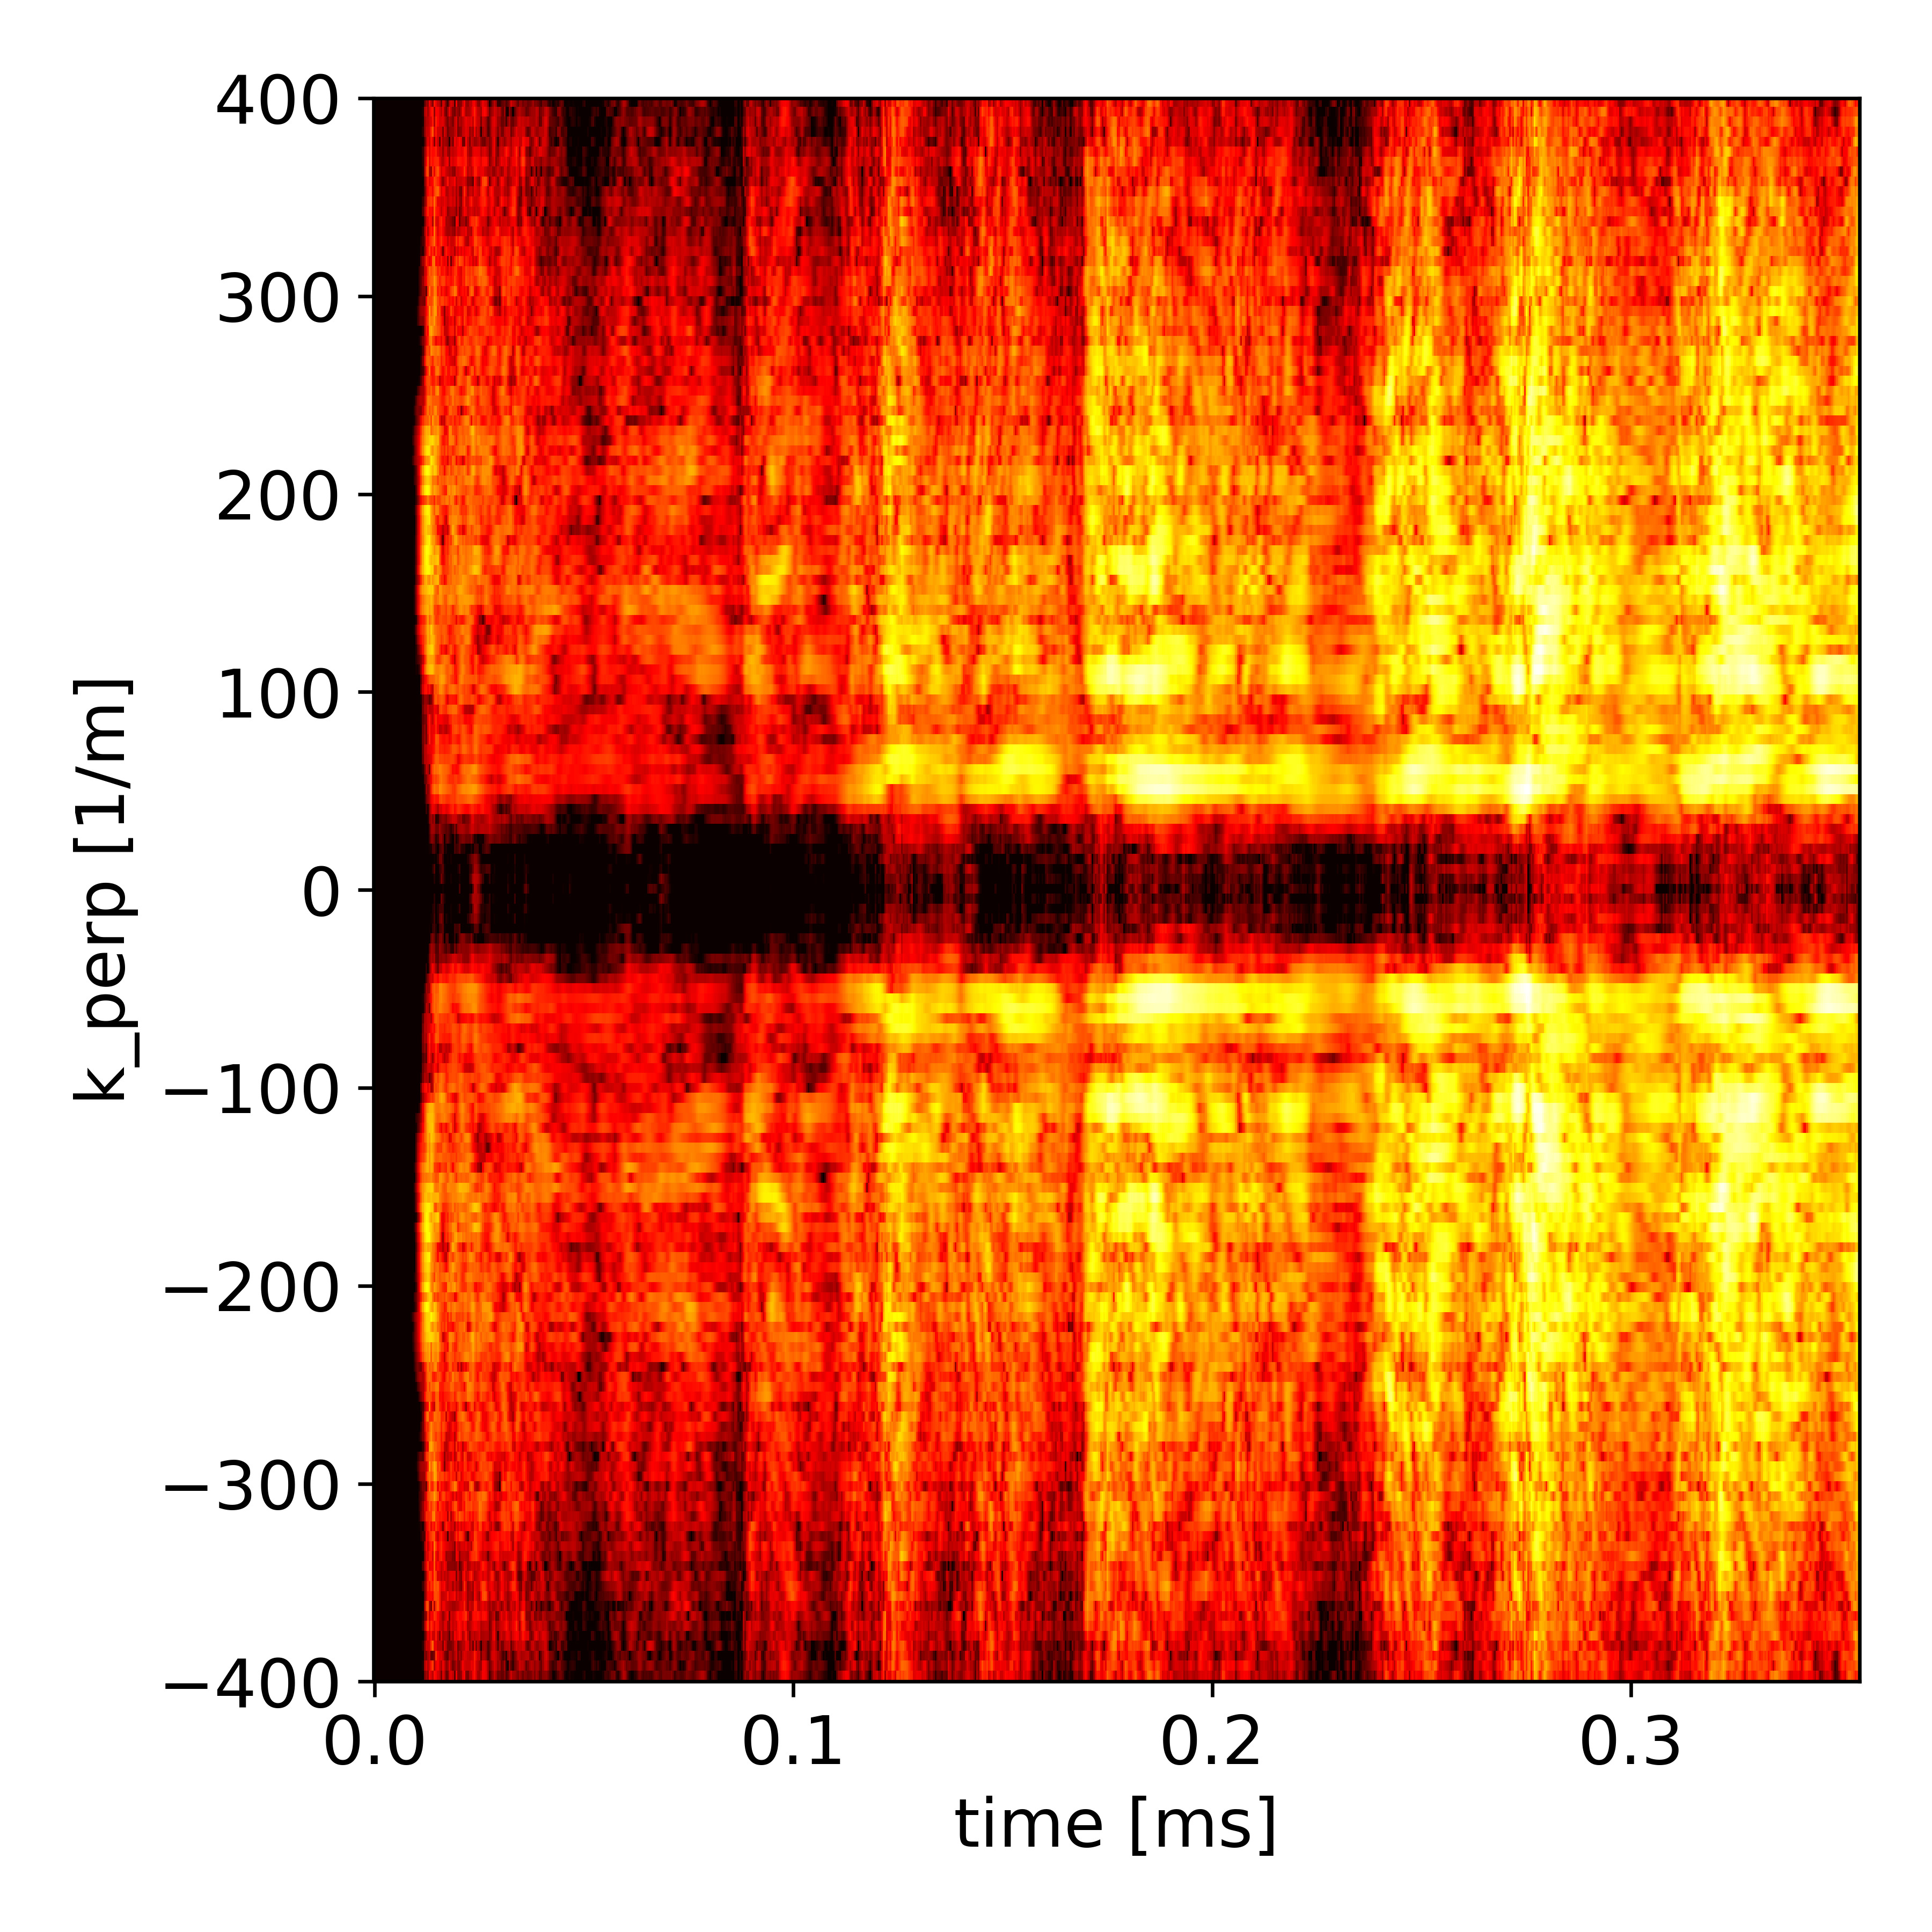
\includegraphics[width=1\textwidth]{schemes/k_perp_time_spec1_n_PHIJ_mass_1.jpg}
		\subcaption{Electron inertia scenario}
		\label{fig:CIRC_evolutionKperp_PHIJ}
	\end{subfigure}
	\begin{subfigure}[t]{0.45\textwidth}
		\centering
		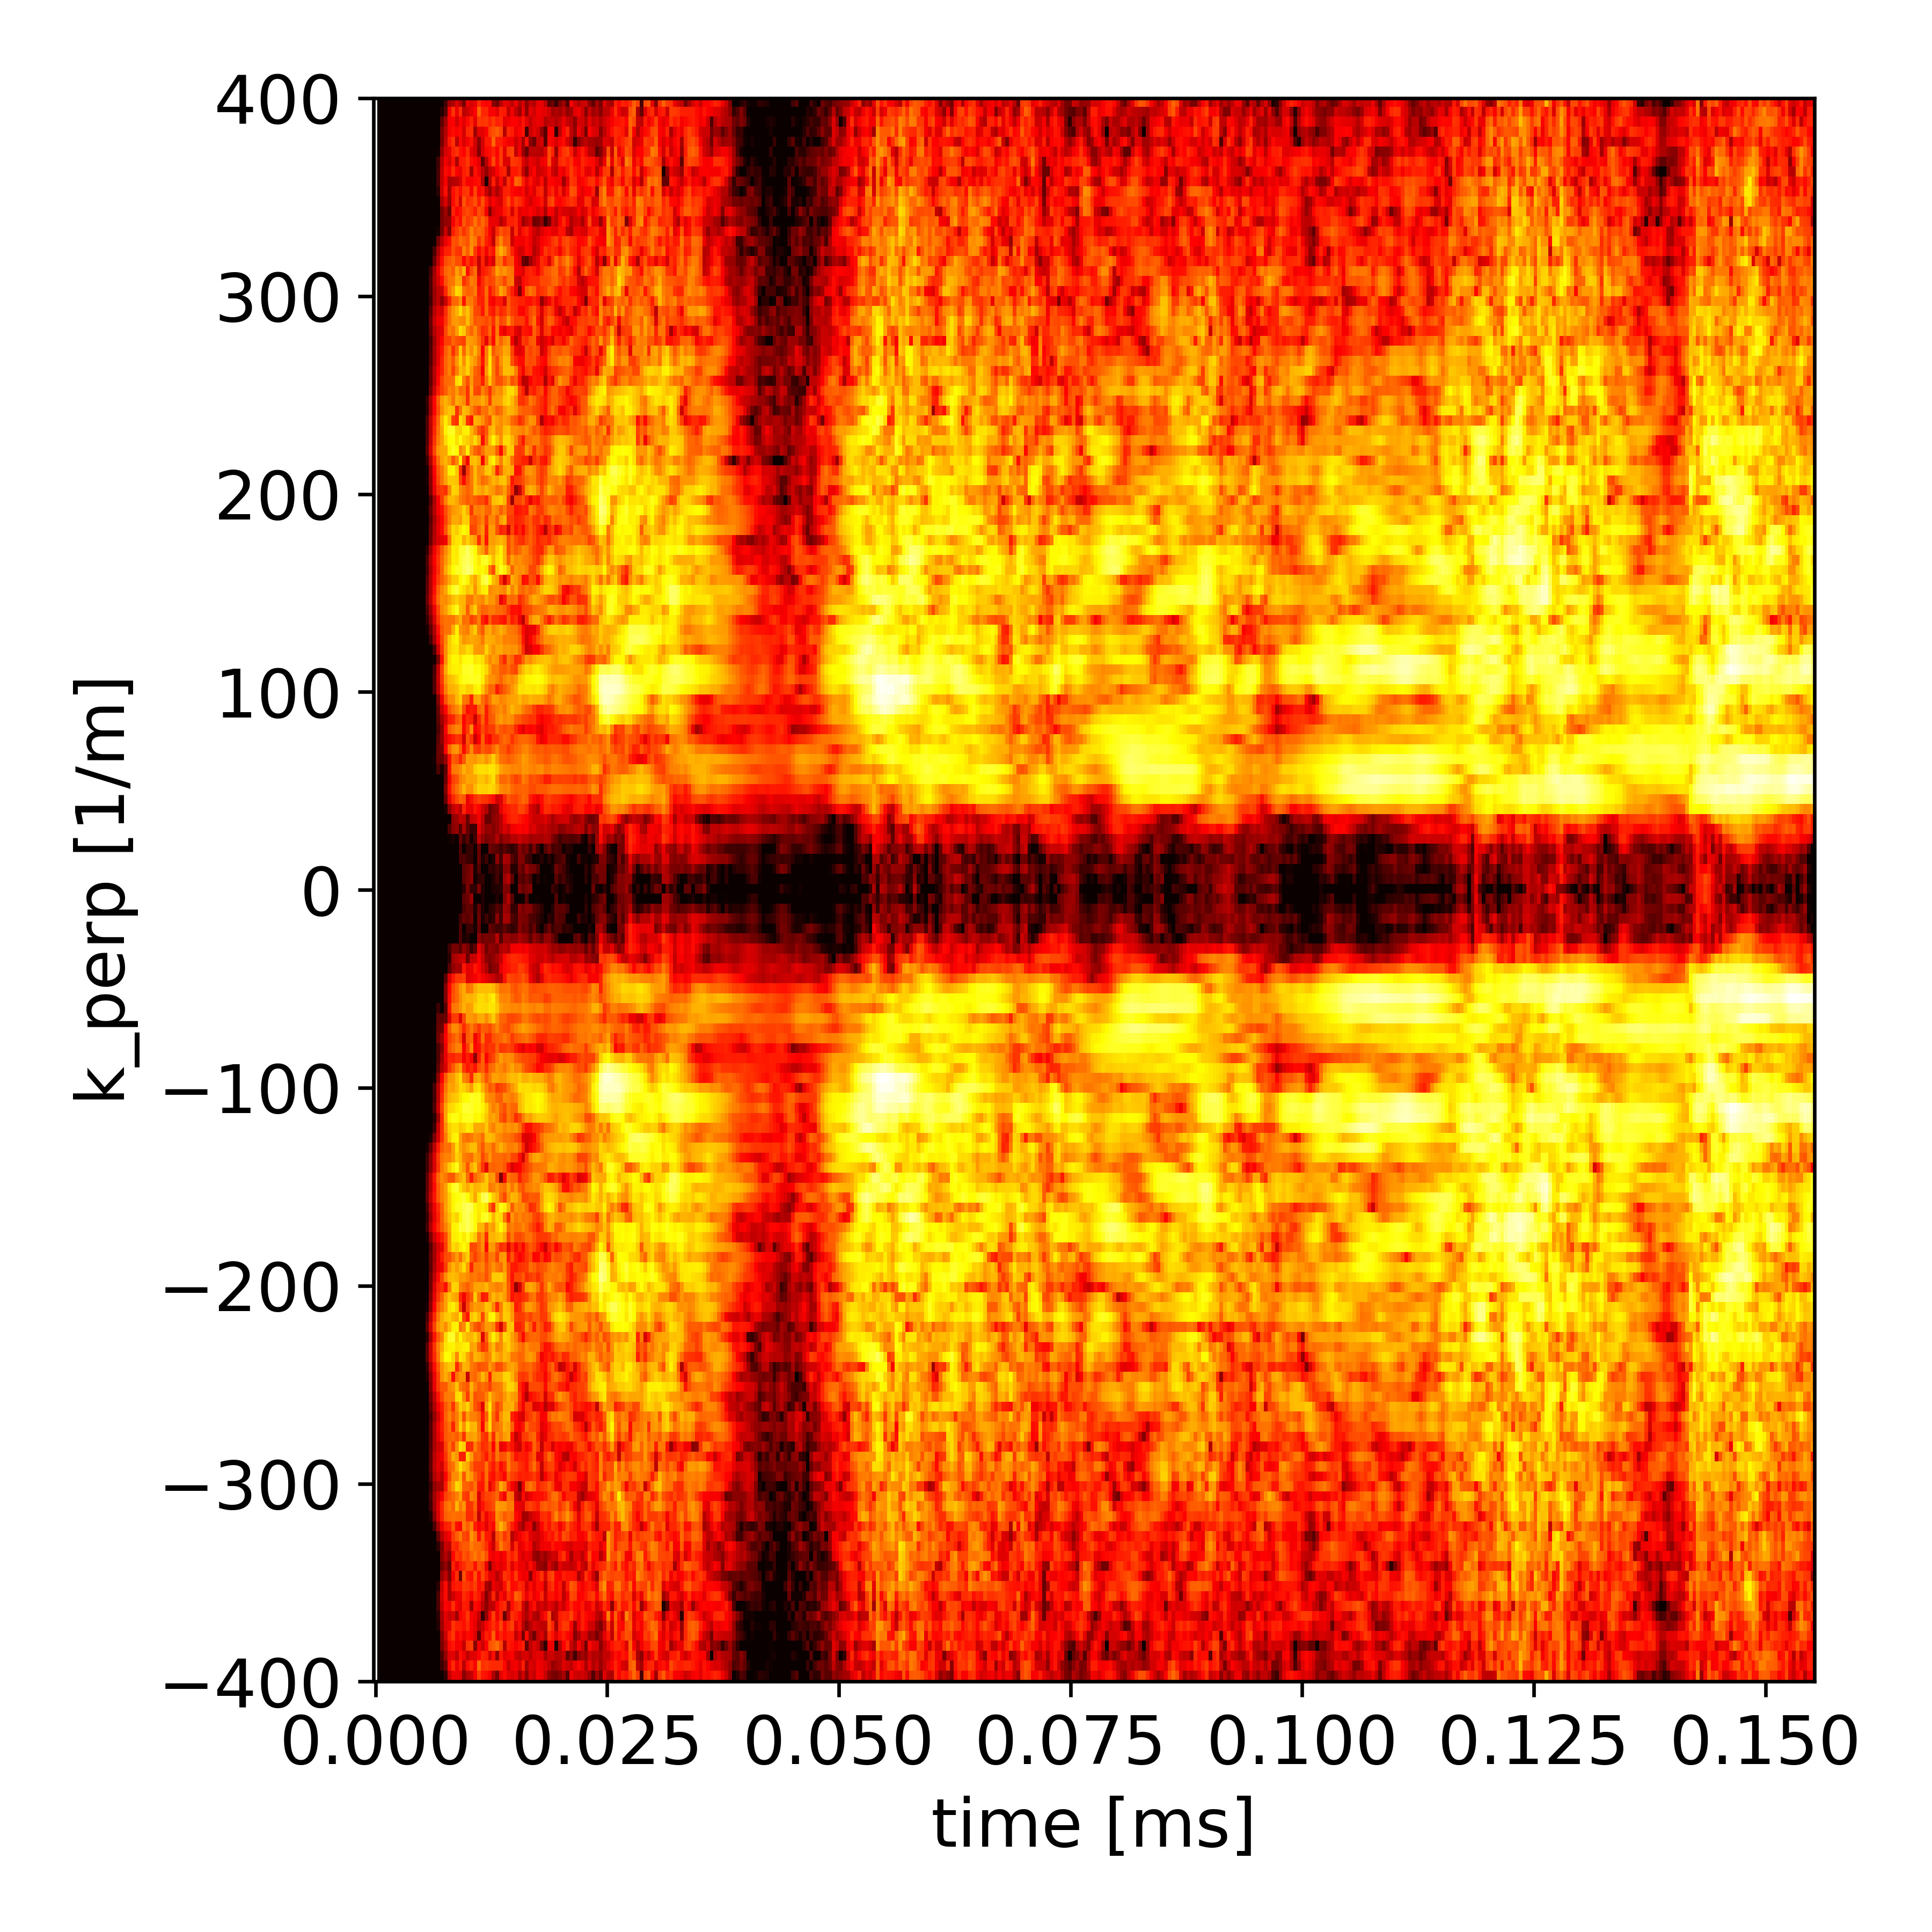
\includegraphics[width=1\textwidth]{schemes/k_perp_time_spec1_n_PHIAJ_beta_1.jpg}
		\subcaption{Inductive electromagnetic scenario}
		\label{fig:CIRC_evolutionKperp_PHIAJ}
	\end{subfigure}
	\caption{Evolution of the power spectrum associated to the perpendicular modes $k_\perp$ over the simulation time. Complement to Fig. \ref{fig:CIRC_evolutionKperp}}
	\label{fig:CIRC_evolutionKperp_bis}
\end{figure}



\section{Flutter field in the low-power TCV scenario}
\label{sec:turbulentProfiles_poincareLmode}


\begin{figure}[H]\centering
	\centering
	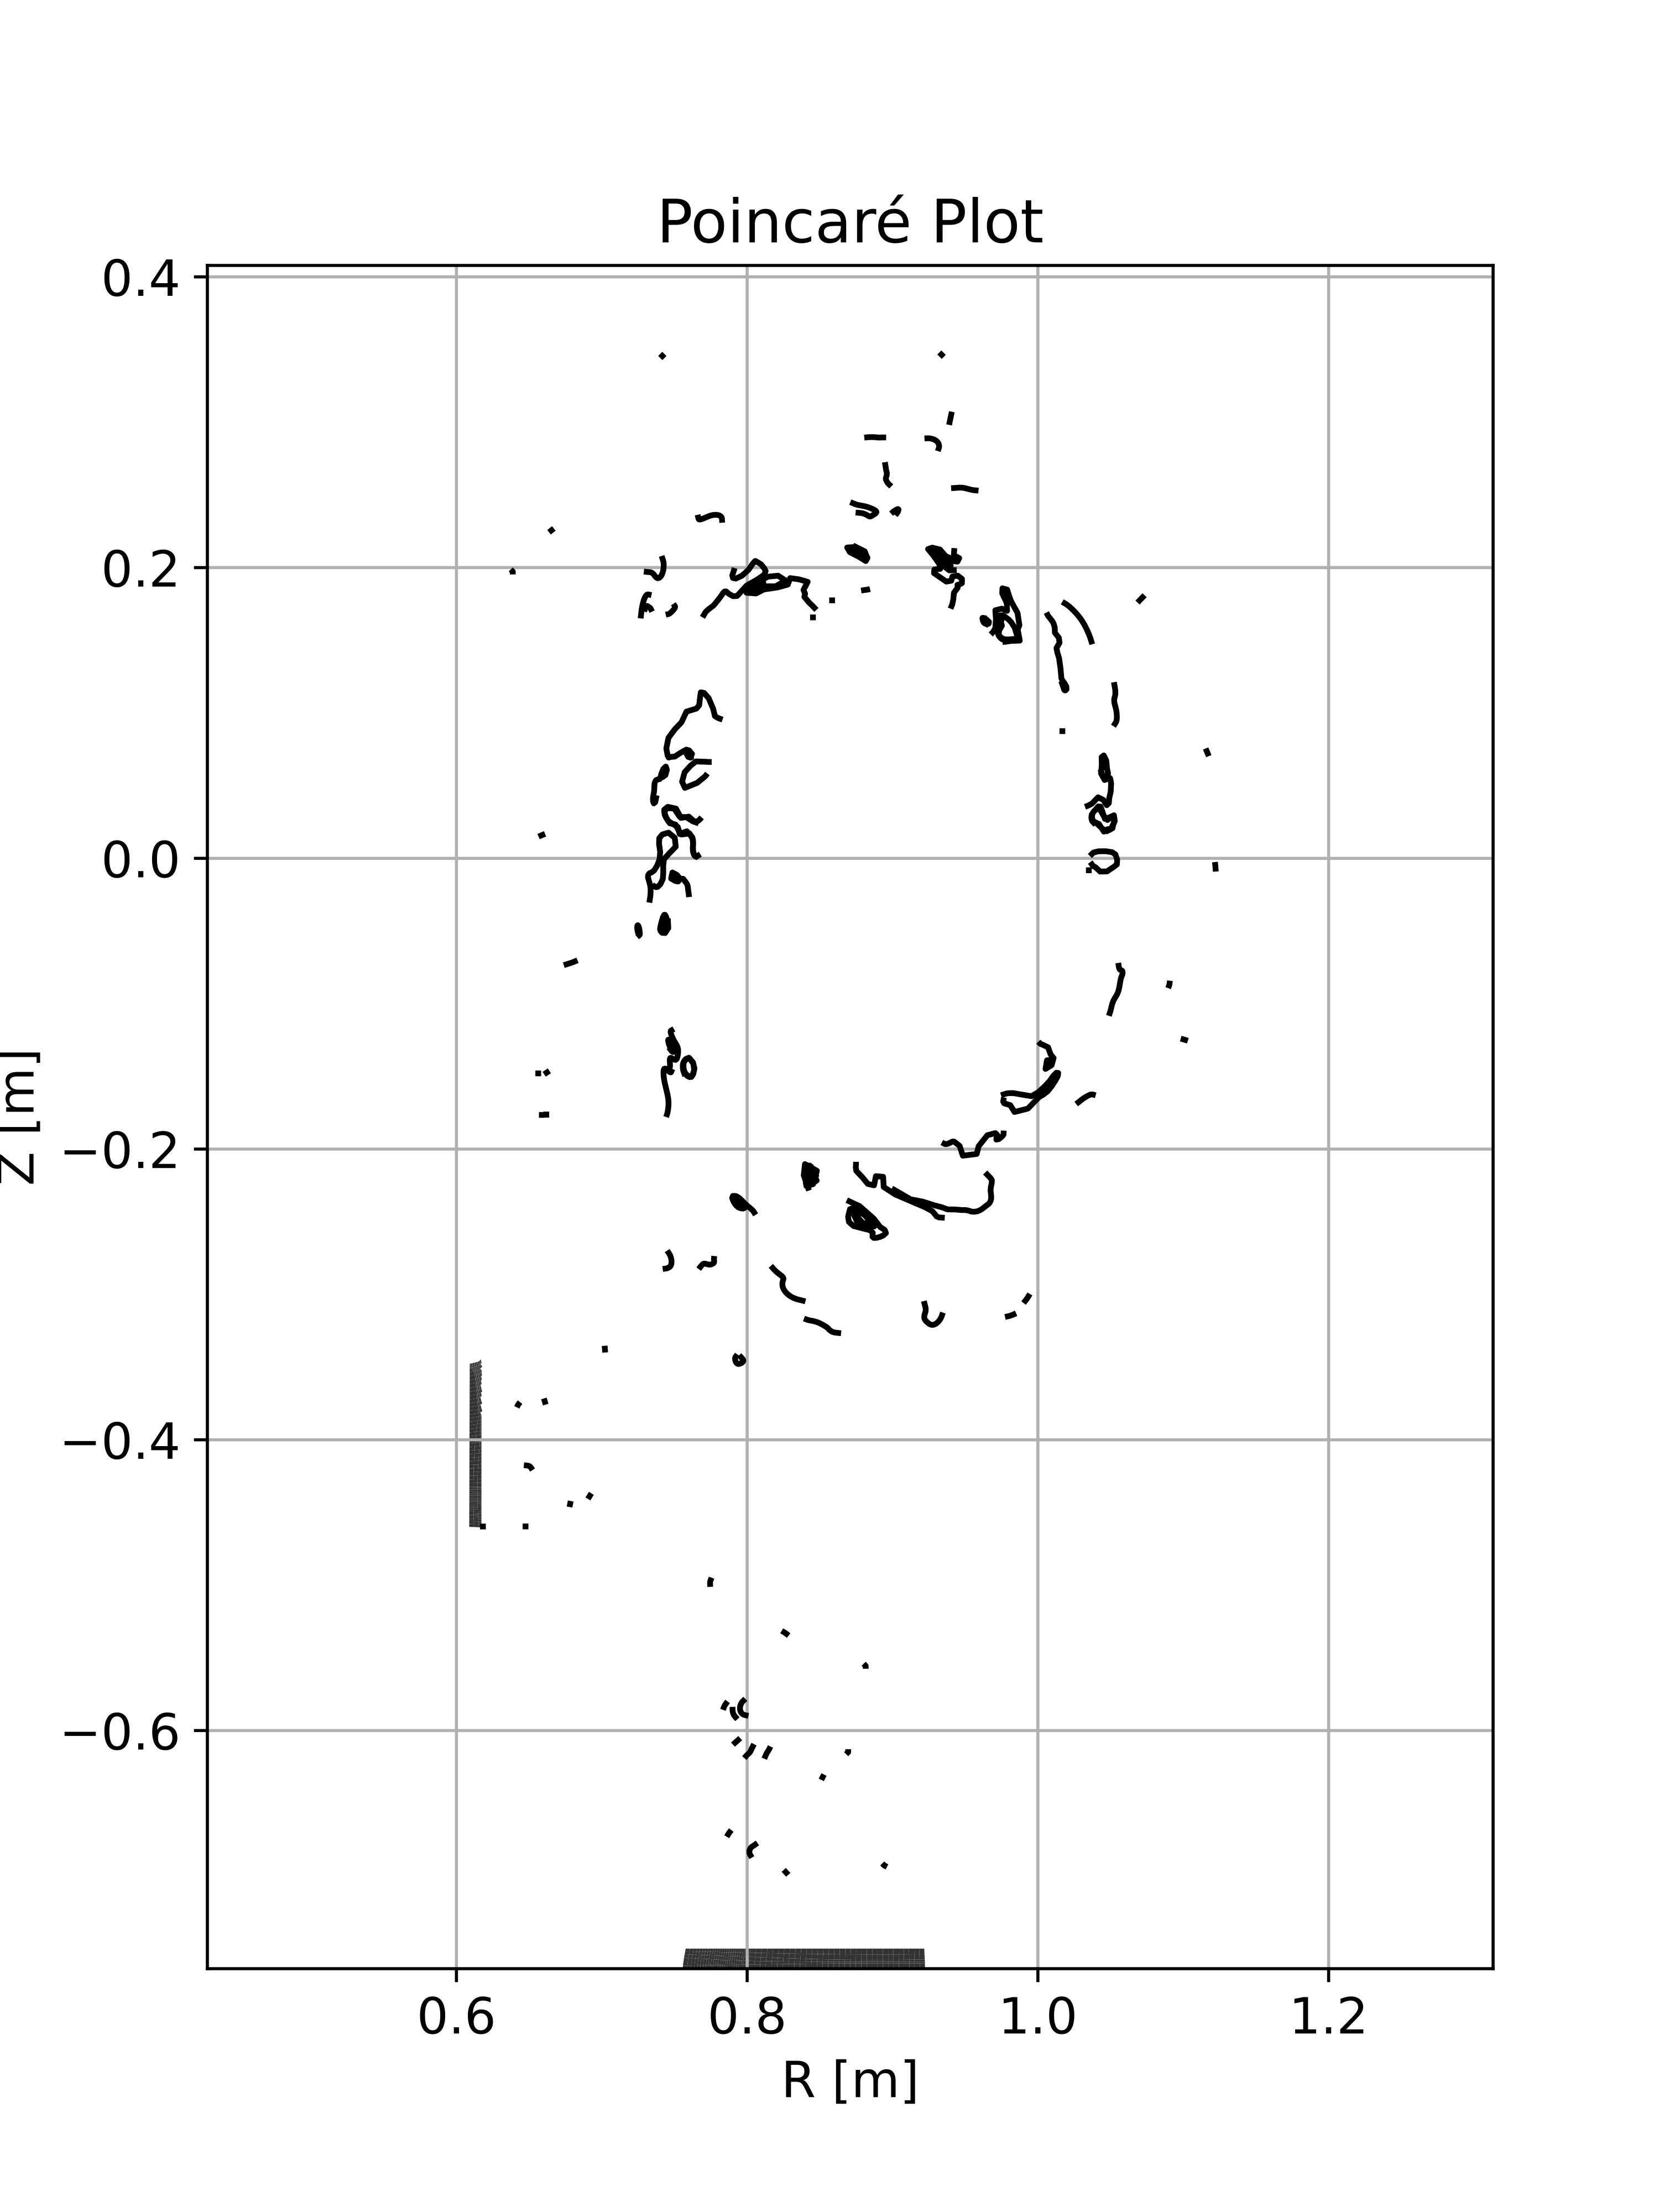
\includegraphics[width=0.6\textwidth]{schemes/poincareTCV_Lmode.jpg}
	\caption{Poincaré plot of the fluctuating magnetic field in the TCV low-power case for a random seed of 500 points in a TCV poloidal plane.}
	\label{fig:TCV_poincareFlutter_Lmode}
\end{figure}


